\documentclass{article}

\usepackage[utf8]{inputenc}

\usepackage{amssymb}
\usepackage{amsmath}
\usepackage{verbatim}
\usepackage{physics}
\usepackage{geometry}
\usepackage{float}
\usepackage{hyperref}
\usepackage{graphicx}
\usepackage{slashed} % Feynman slash notation
\usepackage{pgfplots}
\usepackage{feynmf} % for feynman diagrams
\usepackage{listings} % for code listings
\usepackage{xcolor}
\usepackage{svg} % svg images

%New colors defined below
\definecolor{codegreen}{rgb}{0,0.6,0}
\definecolor{codegray}{rgb}{0.5,0.5,0.5}
\definecolor{codeblue}{rgb}{0.4,0.84,0.93}
\definecolor{backcolour}{rgb}{0.95,0.95,0.92}

%Code listing style named "codestyle"
\lstdefinestyle{codestyle}{
    backgroundcolor=\color{backcolour},   
    commentstyle=\color{codegreen},
    keywordstyle=\color{magenta},
    numberstyle=\tiny\color{codegray},
    stringstyle=\color{codeblue},
    basicstyle=\ttfamily\footnotesize,
    breakatwhitespace=false,         
    breaklines=true,                 
    captionpos=b,                    
    keepspaces=true,                 
    numbers=left,                    
    numbersep=5pt,                  
    showspaces=false,                
    showstringspaces=false,
    showtabs=false,                  
    tabsize=2
}

\lstset{style=codestyle}

\newcommand{\eqname}[1]{\tag*{#1}}% Tag equation with name
\newcommand{\qwdots}{\ar@{.}[]+<-1em,0em>;[]+<0em,0em>}

\usepackage{tikz}
\usetikzlibrary{tikzmark} % arrow pointing to character in equation https://tex.stackexchange.com/questions/191217/arrow-pointing-to-subscript-in-equation

\usepackage[bottom]{footmisc} % put footnote at the bottom of the page https://tex.stackexchange.com/questions/9425/how-to-fix-footnote-position-at-the-bottom-of-the-page

\usepackage[
    type={CC},
    modifier={by-sa},
    version={4.0}
]{doclicense}

\usepackage{amsthm}
\theoremstyle{definition}
\newtheorem{definition}{Definition}[section]
\newtheorem{theorem}{Theorem}[section]
\newtheorem{corollary}{Corollary}[theorem]
\newtheorem{lemma}[theorem]{Lemma}
\newtheorem{prop}[theorem]{Proposition}
\newtheorem{example}{Example}[section]

\allowdisplaybreaks % page breaks in equations
\graphicspath{{./img/}{./plots/}}

\geometry{
  a4paper,
  left=29mm,
  right=29mm,
  top=20mm,
}

\def\code#1{\texttt{#1}}

\title{Proseminar on Computational Methods in QFT \\ Berends Giele Recursion \\ Report}
\author{Roman Gruber}
\date{ETH Zürich, October 2019}

\numberwithin{equation}{section}
\begin{document}

\maketitle

\abstract 
QCD tree amplitudes are of great interest. A calculation of tree level scattering amplitudes in QCD with only gluons involved is presented. The calculation is simplified using color decomposition of full amplitudes into color ordered partial amplitudes. The results are formulated using the spinor helicity formalism for massless vector bosons. A concrete implementation of the methods mentioned in the report are introduced and further ways for optimisation are discussed.
\newline

\doclicenseThis

\noindent\textcolor{gray}{\hrulefill}

\tableofcontents

\noindent\textcolor{gray}{\hrulefill}

\section{Introduction}

For predictions of multi-jet processes at high-energy colliders, we need the knowledge of scattering amplitudes with multiple final parton states in QCD. They are evident in the prediction of cross sections. Writing down all involved Feynman diagrams in the perturbative expansion for such a process can become very cumbersome, since they are armed with a complicated color algebra any many kinematic variables. The perturbative expansion is in the QCD couping $\alpha_s$, which is in the applicable scale at high energies \cite{deur2016}. In this report such amplitudes are discussed at tree level with an arbitrary number of gluons.

In section \ref{sec:spinor} the spinor helicity formalism for massless vector bosons is briefly introduced, such that later in the report, we are able to correctly formulate the problems. It turns out that MHV amplitudes can be simplified massively using that formalism.

In a second preliminary in section \ref{sec:colorordering} a concept called color ordering is introduced. With it, we can decompose tree level amplitudes into parts that are not dependent on color anymore. These parts are then called color ordered amplitudes or partial amplitudes. Such objects have much simpler kinematic properties than the full amplitude, since they only recieve contributions from diagrams with a particular ordering of the external legs. The remaining components of the full amplitude consist of pure traces that can be evaluted quite fast.

Section \ref{sec:bgcurrent} the Berends-Giele current is presented. This is a recursive approach to calculate partial amplitudes. Even if the analytical expressions recieved by this method are not easy to simplify, the numerical implementation is simple and evaluation is quite efficient.

In section \ref{sec:pt} a formula for MHV amplitudes is introduced and proofed - the Parke-Taylor formula. MHV amplitudes are maximally helicity violating amplitudes that are not vanishing. In case of pure gluonic scattering amplitudes, they consist of $n-2$ gluons with the same helicity and $2$ with the opposite helicity.

Evetually in section \ref{sec:implementation} a concrete implementation of both - the Berends-Giele current and the Parke-Taylor formula - is discussed. Both formulas are compared in terms of performace. The computation time required by these two methods scales with the number of external legs. The linear scaling of the Parke-Taylor formula of course ends up in a faster calculation than with the Berends-Giele recursion which scales with $n!$, because it's recursive. 

Finally in the appendices there are - for the sake of completeness - Feynman rules for QCD with and without color ordering in Feynman gauge.

\section{The Spinor helicity formalism for massless vector bosons}
\label{sec:spinor}

In calculating amplitudes in QCD one question that arises is: What are the right kinematic variables for scattering amplitudes? Typically one uses the 4-momenta of the involved particles. For the momenta, specially their Lorentz-invariant products $s_{ij} = \left( p_i + p_j \right)^2$ should be considered. Also the helicity basis \cite{berends81} is very convenient, where the spin is quantized along the axis of the momentum $p$. For positive helicity, the spin points in the same direction as $p$, for negtive helicity in the opposite direction. We have $u_{\pm}(p)$, which is a $4$-spinor. We know that for massless vectors there is a smaller representation which is two dimensional. For a four momentum $p$ and a helicity $h$, we get two $2$-spinors:

\begin{align*}
    p^{\mu}, h \rightarrow u_{-}(p) &= \begin{pmatrix} \lambda_{p \alpha} \\ 0 \\ 0\end{pmatrix} \leftrightarrow | p \rangle = \lambda_{p \alpha} = \begin{pmatrix}\cdot \\ \cdot\end{pmatrix} \\
    u_{+}(p) &= \begin{pmatrix}0 \\ 0 \\ \tilde{\lambda}_{p}^{\dot{\alpha}} \end{pmatrix} \leftrightarrow | p \rbrack = \tilde{\lambda}^{\dot{\alpha}}_p = \begin{pmatrix}\cdot \\ \cdot\end{pmatrix}.
\end{align*}

In this representation, $| p \rangle$ is a column vector with helicity $-1/2$, whereas $| p \rbrack$ is a column vector with helicity $+1/2$. The dotted and undotted indices correspond to two different spinor representations of the Lorentz-group. Positive $u_{\pm}$ and negative $v_{\pm}$ energy solutions are not distinct, since $p^2 = 0$.

Using this formalism, the massless Dirac equation can then be written as

\begin{align*}
    \slashed{p} | p \rangle = \slashed{p} | p \rbrack = 0.
\end{align*}

\begin{definition}[Short notation of spinors]

As a short notation, when we are dealing with $n$ particles, we have $n$ four momenta labelled $p_i$, helicities labelled $h_i$ and maybe adjoint colors labelled $a_i$, where $i \in \{1, ..., n\}$. The $i$-th spinor can then be written as

\begin{align*}
    | p_i \rangle \equiv | i \rangle, \\
    | p_i \rbrack \equiv | i \rbrack.
\end{align*}

\end{definition}

Next, we want to build some Lorentz-invariant quantities and define the spinor product.

\begin{definition}[Spinor product]
\label{def:spinor_product}

The spinor product can be performed between spinors of the same representation

\begin{align*}
    \langle ij \rangle &\equiv \lambda^{\alpha}_i \epsilon_{\alpha \beta} \lambda^{\beta}_j, \\
    \lbrack ij \rbrack &\equiv \tilde{\lambda}_{i \dot{\alpha}} \epsilon^{\dot{\alpha} \dot{\beta}} \tilde{\lambda}_{j \dot{\beta}},
\end{align*}

where the $\epsilon$ matrices are anti-symmetric and given by

\begin{align*}
    \epsilon_{\alpha \beta} = \epsilon_{\dot{\alpha} \dot{\beta}} &= \begin{pmatrix}0 & -1 \\ 1 & 0\end{pmatrix}, & \epsilon^{\alpha \beta} = \epsilon^{\dot{\alpha} \dot{\beta}} &= \begin{pmatrix}0 & 1 \\ -1 & 0\end{pmatrix}.
\end{align*}

Notice that, the spinor products are anti-symmetric by definition, $\langle ii \rangle = \lbrack ii \rbrack = 0$.

\end{definition}

\begin{definition}[Momentum products and sums]

To deal with multiple momenta later, we define some intermediate quantities

\begin{align}
     P_{i,j} &= p_i + \dots + p_j, \\
     s_{ij} &= \left( p_i + p_j \right)^2.
\end{align}

\end{definition}

\begin{definition}[Pauli matrices]

The Pauli matrices are defined as

\begin{align*}
    \sigma^0 &= 
    \begin{pmatrix}
        1 & 0 \\
        0 & 1
    \end{pmatrix}, &
    \sigma^1 &= 
    \begin{pmatrix}
        0 & 1 \\
        1 & 0
    \end{pmatrix}, &
    \sigma^2 &= 
    \begin{pmatrix}
        0 & -i \\
        i & 0
    \end{pmatrix}, &
    \sigma^3 &= 
    \begin{pmatrix}
        1 & 0 \\
        0 & -1
    \end{pmatrix},
\end{align*}

and

\begin{align*}
    \sigma^{\mu} &= (1, \sigma^1, \sigma^2, \sigma^3), \\
    \overline{\sigma}^{\mu} &= (1, -\sigma^1, -\sigma^2, -\sigma^3).
\end{align*}

\end{definition}

\subsection{Important identities and definitions}

Using the formalism defined above, there are now some identities that follow.

\begin{lemma}[Fierz identity]

\begin{align}
    \langle i | \sigma^{\mu} | j \rbrack \langle k | \sigma_{\mu} | l \rbrack &= 2 \langle ik \rangle \lbrack lj \rbrack \label{eq:fierz} 
\end{align}

\end{lemma}

\begin{lemma}[Charge conjugation identity]

\begin{align}
    \langle i | \sigma^{\mu} | j \rbrack &= \lbrack j | \overline{\sigma}^{\mu} | i \rangle \label{eq:ijji}
\end{align}

\end{lemma}

\begin{lemma}[Schouten identity]

\begin{align}
    \langle ij \rangle \bra{k} + \langle jk \rangle \bra{i} + \langle ki \rangle \bra{j} = 0 \label{eq:schouten}
\end{align}

\end{lemma}

\begin{lemma}[Squaring identity]

\begin{align}
     \langle ij \rangle \lbrack ji \rbrack = 2 p_i \cdot p_j = s_{ij} \label{eq:ij}
\end{align}

\end{lemma}

\begin{definition}[Feynman slash notation]

Feynmans slash notation has also a representation in the new formalism

\begin{align}
     \slashed{p} = \sigma^{\mu} p_{\mu} = p^{\mu} \sigma_{\mu} = | p \rangle \lbrack p | + | p \rbrack \langle p |. \label{eq:slash}
\end{align}

\end{definition}

Using the spinor products, we are now able to build polarisation vectors for massless vector bosons with helicity $h=\pm1$ \cite{xu86},

\begin{align}
    \varepsilon_{+}^{\mu}(p,q) = \frac{1}{\sqrt{2}} \frac{\langle q | \sigma^{\mu} | p \rbrack }{ \langle qp \rangle } \quad \text{and} \quad \varepsilon_{-}^{\mu}(p,q) = - \frac{1}{\sqrt{2}} \frac{\lbrack q | \overline{\sigma}^{\mu} | p \rangle }{ \lbrack qp \rbrack }, \label{eq:polvecs}
\end{align}

where $q$ is a reference vector with massless momentum $q^2 = 0$. $\varepsilon_{+}$ is a state with helicity $h=+1$, because $| p \rbrack$ in the numerator gives $+1/2$ and $| p \rangle$ gives $-1/2$, but in the denominator it also gives $+1/2$. The choice of $q$ is a gauge choice and absolutely free as long as $q^2=0$ and $q$ is not proportional to $p$, because else the spinor product in the denominator would vanish. This choice originates from the gauge invariance of the gauge field $A^a_{\mu}$ in the Lagrangian. The results in the end should not depend on any reference momentum $q$, but intermediate results do in general. When choosing a different $q'$ as reference momentum, the polarisation vectors are shifted by an amount proportional to $p^{\mu}$.

\section{Color Ordering}
\label{sec:colorordering}

Color ordering is a concept to treat the color component of scattering amplitudes. We want to decompose the problem into subproblems. This can be achieved by color ordering. In the Feynman rules of QCD, there is a lot of color dependency (see appendix \ref{sec:frules}).

\subsection{QCD gauge group}

The gauge group of QCD is $SU(N_c)$ - unitary $N_c \times N_c$ matrices with unit determinant - with $N_c = 3$ the number of colors. The Lie algebra of this group is $\mathfrak{su}(N_c)$ - traceless hermitian $N_c \times N_c$ matrcies. The unit determinant converts to tracelessness, when going to the Lie algebra. The dimension of both the gauge group and its Lie algebra is $N_c^2 - 1$ (the tracelessness condition removes one dimention). We therefore have a basis of the Lie algebra - the generators of the gauge group - denoted by $T^a$, where $a$ is the adjoint color index going from $1$ to $N_c^2 - 1 = 8$.

\begin{definition}[Normalisation]
\label{def:normalisation}
We define the normalisation of the generators as

\begin{align}
    tr (T^a T^b) = \delta^{ab}. \label{eq:normalisation}
\end{align}

This normalisation, though uncommon in literature, prevents later expressions from unnecessary $\sqrt{2}$ apprearing.

\end{definition}

\begin{prop}[Fierz identity]
\label{prop:fierz}

The generators $T^a$ of the gauge group satisfy the following identity \cite{bg87colorordering}:

\begin{align}
    {\left( T^a \right)_{i_1}}^{\bar{\jmath}_1} {\left( T^a \right)_{i_2}}^{\bar{\jmath}_2} = {\delta_{i_1}}^{\bar{\jmath}_2} {\delta_{i_2}}^{\bar{\jmath}_1} - \frac{1}{N_c} {\delta_{i_1}}^{\bar{\jmath}_1} {\delta_{i_2}}^{\bar{\jmath}_2} \label{eq:fierz2} 
\end{align}

\end{prop}

\begin{proof}

Equation \eqref{eq:fierz2} is just the statement that the $T^a$ together with the identity form a basis of the $N_c \times N_c$ hermitian matrices. The $T^a$ are a basis of $N_c \times N_c$ traceless hermitian matrices, since the identity is linearly indepdenant of all $T^a$. An arbitrary hermitian matrix $A$ can therefore be written as

\begin{align*}
    A = \sum_{a=1}^{N_c^2 -1} b_a T^a + b_n id,
\end{align*}

where $n=N_c^2$. We now apply the trace on both sides of that equation:

\begin{align*}
    tr \left( A \right) = b_n N_c,
\end{align*}

where we have used the fact that the $T^a$ are traceless and the trace of the identity is its dimension. We obtain the $n$-th coefficient $b_n = tr \left( A \right) /N_c$. We can also multiply both sides with $T^c$ and then take the trace and obtain the remaining coefficients:

\begin{align*}
    tr \left( A T^c \right) = b_c,
\end{align*}

where we again used the tracelessness of the $T^a$ and their normalisation (definition \ref{def:normalisation}). Therefore we can write the $i,j$-th entry of the matrix $A$ as

\begin{align*}
    {A_{i}}^{j} = \sum_{a=1}^{N_c^2 -1} {(T^a)_{k}}^{l} {A_{l}}^{k} {(T^a)_{i}}^{j} + \frac{tr \left( A \right)}{N_c} {\delta_{i}}^{j}.
\end{align*}

Using $tr \left( A \right) = tr \left( A id \right) = {A_{l}}^{k} {\delta_{k}}^{l}$ and ${A_{i}}^{j} = {A_{l}}^{k} {\delta_i}^l {\delta_j}^k$, we find

\begin{align*}
    {A_{l}}^{k} \left[ \sum_{a=1}^{N_c^2 -1} {(T^a)_k}^l {(T^a)_i}^j + \frac{1}{N_c} {\delta_k}^l {\delta_i}^j - {\delta_i}^l {\delta_j}^k \right] = 0,
\end{align*}

that holds for all ${A_{l}}^{k}$, which implies that the term is the square backets must be $0$.

\end{proof}

On the other hand, the generators also satisfy the relation

\begin{align}
    [ T^a, T^b ] = i \sqrt{2} \sum_{c=1}^{N_c^2 - 1} f^{abc} T^c, \label{eq:liebracket}
\end{align}

where the $f^{abc}$ are the anti-symmetric structure constants. The above relation can be solved for the $f^{abc}$: starting with equation \eqref{eq:liebracket} and multiplying from the right side with another $T^d$ and taking the trace, we obtain

\begin{align}
    tr (T^a T^b T^d) - tr(T^b T^b T^d)  = i \sqrt{2} \sum_{c=1}^{N_c^2 - 1} f^{abc} tr (T^c T^d).
\end{align}

Using the definition of the normalisation \ref{def:normalisation}, the sum on the right hand side is over a Kronecker delta, therefore only one term is not vanishing

\begin{align}
    f^{abc} = -\frac{i}{\sqrt{2}} \left( tr (T^a T^b T^c) - tr(T^b T^b T^c) \right). \label{eq:fabc}
\end{align}

The expression for the structure constants \eqref{eq:fabc} can be written pictorially in a very intuitive way taking only the color component from the Feynman rules into account:

\begin{equation}
\begin{aligned}
    &\begin{gathered}
        \begin{fmffile}{report_diagram_fabc1}
        \fmfframe(0,10)(0,10){
        \begin{fmfgraph*}(50,40)
            \fmfstraight
            \fmfset{arrow_len}{2mm}
            \fmfset{curly_len}{2mm}
            \fmfset{thin}{0.8pt}
            \fmfpen{thin}
            \fmftop{g2}
            \fmfbottom{g1,g3}
            \fmf{gluon}{g1,v}
            \fmf{gluon}{g2,v}
            \fmf{gluon}{g3,v}
            \fmflabel{$a$}{g1}
            \fmflabel{$b$}{g2}
            \fmflabel{$c$}{g3}
        \end{fmfgraph*}
        }
        \end{fmffile}
    \end{gathered}&
    &=&
    &\begin{gathered}
        \begin{fmffile}{report_diagram_fabc2}
        \fmfframe(0,10)(0,10){
        \begin{fmfgraph*}(50,40)
            \fmfstraight
            \fmfset{arrow_len}{2mm}
            \fmfset{curly_len}{2mm}
            \fmfset{thin}{0.8pt}
            \fmfpen{thin}
            \fmftop{g2}
            \fmfbottom{g1,g3}
            \fmf{gluon}{g1,v1}
            \fmf{gluon}{g2,v2}
            \fmf{gluon}{g3,v3}
            \fmf{fermion,label=$i$,left=0.6,tension=0.7}{v1,v2}
            \fmf{fermion,label=$j$,left=0.6,tension=0.7}{v2,v3}
            \fmf{fermion,label=$k$,left=0.6,tension=0.7}{v3,v1}
            \fmflabel{$a$}{g1}
            \fmflabel{$b$}{g2}
            \fmflabel{$c$}{g3}
        \end{fmfgraph*}
        }
        \end{fmffile}
    \end{gathered}&
    &-&
    &\begin{gathered}
        \begin{fmffile}{report_diagram_fabc3}
        \fmfframe(0,10)(0,10){
        \begin{fmfgraph*}(50,40)
            \fmfstraight
            \fmfset{arrow_len}{2mm}
            \fmfset{curly_len}{2mm}
            \fmfset{thin}{0.8pt}
            \fmfpen{thin}
            \fmftop{g2}
            \fmfbottom{g1,g3}
            \fmf{gluon}{g1,v1}
            \fmf{gluon}{g2,v2}
            \fmf{gluon}{g3,v3}
            \fmf{fermion,label=$i$,right=0.6,tension=0.7}{v2,v1}
            \fmf{fermion,label=$j$,right=0.6,tension=0.7}{v3,v2}
            \fmf{fermion,label=$k$,right=0.6,tension=0.7}{v1,v3}
            \fmflabel{$a$}{g1}
            \fmflabel{$b$}{g2}
            \fmflabel{$c$}{g3}
        \end{fmfgraph*}
        }
        \end{fmffile}
    \end{gathered}& \\
    &i \sqrt{2} f^{abc}&
    &=&
    &{(T^a)_k}^{\bar{\imath}} {(T^b)_i}^{\bar{\jmath}} {(T^c)_j}^{\bar{k}} &
    &-&
    &{(T^a)_i}^{\bar{k}} {(T^b)_j}^{\bar{\imath}} {(T^c)_k}^{\bar{\jmath}}& \\
    &i \sqrt{2} f^{abc}&
    &=&
    &tr ( T^a T^b T^c )&
    &-&
    &tr ( T^a T^c T^b ).& \label{eq:fd:fabc}
\end{aligned}
\end{equation}

The structure constant $f^{abc}$ is proportional to the $3$-gluon vertex according to the Feynman rules (see appendix \ref{sec:frules}), whereas the loop diagrams on the right hand side produce traces of all involved generators $T^a$ using the Feynman rule for the quark-gloun vertex. The Fierz identity \eqref{eq:fierz2} can also be illustrated in a similar way:

\begin{equation}
\begin{aligned}
    &\begin{gathered}
        \begin{fmffile}{report_diagram_fierz1}
        \fmfframe(0,10)(0,10){
        \begin{fmfgraph*}(40,20)
            \fmfstraight
            \fmfset{arrow_len}{2mm}
            \fmfset{curly_len}{2mm}
            \fmfset{thin}{0.8pt}
            \fmfpen{thin}
            \fmfleft{f1,f2}
            \fmfright{f3,f4}
            \fmf{fermion,right=0.4,tension=1.0}{f1,v1,f2}
            \fmf{fermion,right=0.4,tension=1.0}{f4,v2,f3}
            \fmf{gluon,label=$a$}{v2,v1}
            \fmflabel{$i_1$}{f1}
            \fmflabel{$\bar{\jmath}_1$}{f2}
            \fmflabel{$\bar{\jmath}_2$}{f3}
            \fmflabel{$i_2$}{f4}
        \end{fmfgraph*}
        }
        \end{fmffile}
    \end{gathered}&
    &=&
    &\begin{gathered}
        \begin{fmffile}{report_diagram_fierz2}
        \fmfframe(0,10)(0,10){
        \begin{fmfgraph*}(40,20)
            \fmfstraight
            \fmfset{arrow_len}{2mm}
            \fmfset{curly_len}{2mm}
            \fmfset{thin}{0.8pt}
            \fmfpen{thin}
            \fmfleft{f1,f2}
            \fmfright{f3,f4}
            \fmf{fermion}{f4,f2}
            \fmf{fermion}{f1,f3}
            \fmflabel{$i_1$}{f1}
            \fmflabel{$\bar{\jmath}_1$}{f2}
            \fmflabel{$\bar{\jmath}_2$}{f3}
            \fmflabel{$i_2$}{f4}
        \end{fmfgraph*}
        }
        \end{fmffile}
    \end{gathered}&
    &-\frac{1}{N_c}&
    &\begin{gathered}
        \begin{fmffile}{report_diagram_fierz3}
        \fmfframe(0,10)(0,10){
        \begin{fmfgraph*}(40,20)
            \fmfstraight
            \fmfset{arrow_len}{2mm}
            \fmfset{curly_len}{2mm}
            \fmfset{thin}{0.8pt}
            \fmfpen{thin}
            \fmfleft{f1,f2}
            \fmfright{f3,f4}
            \fmf{fermion,right=0.4,tension=1.0}{f1,v1,f2}
            \fmf{fermion,right=0.4,tension=1.0}{f4,v2,f3}
            \fmf{phantom}{v1,v2}
            \fmflabel{$i_1$}{f1}
            \fmflabel{$\bar{\jmath}_1$}{f2}
            \fmflabel{$\bar{\jmath}_2$}{f3}
            \fmflabel{$i_2$}{f4}
        \end{fmfgraph*}
        }
        \end{fmffile}
    \end{gathered}& \\
    &{(T^a)_{i_1}}^{\bar{\jmath}_1} {(T^a)_{i_2}}^{\bar{\jmath}_2}&
    &=&
    &{\delta_{i_1}}^{\bar{\jmath}_2} {\delta_{i_2}}^{\bar{\jmath}_1}&
    &-\frac{1}{N_c}&
    &{\delta_{i_1}}^{\bar{\jmath}_1} {\delta_{i_2}}^{\bar{\jmath}_2}.& \label{eq:fd:fierz}
\end{aligned}
\end{equation}

Again the Feynman rules from appendix \ref{sec:frules} where used to derive the pictures. The two equations can therfore be used to rewrite some guonic amplitudes. Let's see this in an example.

\subsection{Color decomposition}

\begin{example}[$4$-gluon vertex]

In this example, we decompose the $4$-gluon vertex into multiple diagrams. We use the two pictorial representations \eqref{eq:fd:fabc} and \eqref{eq:fd:fierz}. The $4$-vertex can be decomposed into $3$ components of each two $3$-vertices by just looking at the Feynman rule:

\begin{equation}
\begin{aligned}
    &\begin{gathered}
        \begin{fmffile}{report_diagram_example_4g1}
        \fmfframe(0,10)(0,10){
        \begin{fmfgraph*}(40,40)
            \fmfstraight
            \fmfset{arrow_len}{1.5mm}
            \fmfset{curly_len}{1.5mm}
            \fmfset{thin}{0.8pt}
            \fmfpen{thin}
            \fmfleft{g1,g2}
            \fmfright{g4,g3}
            \fmf{gluon}{g1,v}
            \fmf{gluon}{g2,v}
            \fmf{gluon}{g3,v}
            \fmf{gluon}{g4,v}
            \fmflabel{$a$}{g1}
            \fmflabel{$b$}{g2}
            \fmflabel{$c$}{g3}
            \fmflabel{$d$}{g4}
        \end{fmfgraph*}
        }
        \end{fmffile}
    \end{gathered}&
    &=&
    &\begin{gathered}
        \begin{fmffile}{report_diagram_example_4g2}
        \fmfframe(0,10)(0,10){
        \begin{fmfgraph*}(40,40)
            \fmfstraight
            \fmfset{arrow_len}{1.5mm}
            \fmfset{curly_len}{1.5mm}
            \fmfset{thin}{0.8pt}
            \fmfpen{thin}
            \fmfleft{g1,g2}
            \fmfright{g4,g3}
            \fmf{gluon}{g1,v1}
            \fmf{gluon}{g2,v1}
            \fmf{gluon}{g3,v2}
            \fmf{gluon}{g4,v2}
            \fmf{gluon,label=$e$}{v2,v1}
            \fmflabel{$a$}{g1}
            \fmflabel{$b$}{g2}
            \fmflabel{$c$}{g3}
            \fmflabel{$d$}{g4}
        \end{fmfgraph*}
        }
        \end{fmffile}
    \end{gathered}&
    &+&
    &\begin{gathered}
        \begin{fmffile}{report_diagram_example_4g3}
        \fmfframe(0,10)(0,10){
        \begin{fmfgraph*}(40,40)
            \fmfstraight
            \fmfset{arrow_len}{1.5mm}
            \fmfset{curly_len}{1.5mm}
            \fmfset{thin}{0.8pt}
            \fmfpen{thin}
            \fmfleft{g1,g2}
            \fmfright{g4,g3}
            \fmf{gluon}{g1,v2}
            \fmf{gluon}{g2,v1}
            \fmf{gluon}{g3,v1}
            \fmf{gluon}{g4,v2}
            \fmf{gluon,label=$e$}{v2,v1}
            \fmflabel{$a$}{g1}
            \fmflabel{$b$}{g2}
            \fmflabel{$c$}{g3}
            \fmflabel{$d$}{g4}
        \end{fmfgraph*}
        }
        \end{fmffile}
    \end{gathered}&
    &+&
    &\begin{gathered}
        \begin{fmffile}{report_diagram_example_4g4}
        \fmfframe(0,10)(0,10){
        \begin{fmfgraph*}(40,40)
            \fmfstraight
            \fmfset{arrow_len}{1.5mm}
            \fmfset{curly_len}{1.5mm}
            \fmfset{thin}{0.8pt}
            \fmfpen{thin}
            \fmfleft{g1,g2}
            \fmfright{g4,g3}
            \fmf{gluon}{g1,v2}
            \fmf{gluon}{g2,v1}
            \fmf{phantom}{g4,v2}
            \fmf{phantom}{g3,v1}
            \fmf{gluon,tension=0}{g3,v2}
            \fmf{gluon,tension=0}{g4,v1}
            \fmf{gluon,label=$e$}{v1,v2}
            \fmflabel{$a$}{g1}
            \fmflabel{$b$}{g2}
            \fmflabel{$c$}{g3}
            \fmflabel{$d$}{g4}
        \end{fmfgraph*}
        }
        \end{fmffile}
    \end{gathered}& \\
    &&
    &&
    &f^{abe} f^{cde}&
    &&
    &f^{ade} f^{bce}&
    &&
    &f^{ace} f^{bde}.&
\end{aligned}
\end{equation}

We decompose the vertex of the first diagram proportional to $f^{abe} f^{cde}$ (the others are analogue)

\begin{align*}
    &\begin{gathered}
        \begin{fmffile}{report_diagram_example_4g5}
        \fmfframe(0,10)(0,10){
        \begin{fmfgraph*}(60,40)
            \fmfstraight
            \fmfset{arrow_len}{2mm}
            \fmfset{curly_len}{2mm}
            \fmfset{thin}{0.8pt}
            \fmfpen{thin}
            \fmfleft{g1,g2}
            \fmfright{g4,g3}
            \fmf{gluon}{g1,v1}
            \fmf{gluon}{g2,v1}
            \fmf{gluon}{g3,v2}
            \fmf{gluon}{g4,v2}
            \fmf{gluon,label=$e$}{v2,v1}
            \fmflabel{$a$}{g1}
            \fmflabel{$b$}{g2}
            \fmflabel{$c$}{g3}
            \fmflabel{$d$}{g4}
        \end{fmfgraph*}
        }
        \end{fmffile}
    \end{gathered}&
    &=&
    &\begin{gathered}
        \begin{fmffile}{report_diagram_example_4g6}
        \fmfframe(0,10)(0,10){
        \begin{fmfgraph*}(60,40)
            \fmfstraight
            \fmfset{arrow_len}{2mm}
            \fmfset{curly_len}{2mm}
            \fmfset{thin}{0.8pt}
            \fmfpen{thin}
            \fmfleft{g1,g2}
            \fmfright{g4,g3}
            \fmf{gluon}{g1,v1}
            \fmf{gluon}{g2,v2}
            \fmf{gluon}{g3,v5}
            \fmf{gluon}{g4,v6}
            \fmf{fermion,left=0.6,tension=0.7}{v1,v2}
            \fmf{fermion,left=0.6,tension=0.7}{v2,v3}
            \fmf{fermion,left=0.6,tension=0.7}{v3,v1}
            \fmf{fermion,left=0.6,tension=0.7}{v4,v5}
            \fmf{fermion,left=0.6,tension=0.7}{v5,v6}
            \fmf{fermion,left=0.6,tension=0.7}{v6,v4}
            \fmf{gluon,label=$e$}{v4,v3}
            \fmflabel{$a$}{g1}
            \fmflabel{$b$}{g2}
            \fmflabel{$c$}{g3}
            \fmflabel{$d$}{g4}
        \end{fmfgraph*}
        }
        \end{fmffile}
    \end{gathered}&
    &\pm \text{permutations}& \\
    & & &=&
    &\begin{gathered}
        \begin{fmffile}{report_diagram_example_4g7}
        \fmfframe(0,10)(0,10){
        \begin{fmfgraph*}(60,40)
            \fmfstraight
            \fmfset{arrow_len}{2mm}
            \fmfset{curly_len}{2mm}
            \fmfset{thin}{0.8pt}
            \fmfpen{thin}
            \fmfleft{g1,g2}
            \fmfright{g4,g3}
            \fmf{gluon}{g1,v1}
            \fmf{gluon}{g2,v2}
            \fmf{gluon}{g3,v5}
            \fmf{gluon}{g4,v6}
            \fmf{plain,left=0.05,tension=0.7}{vi1,v1}
            \fmf{fermion,left=0.6,tension=0.7}{v1,v2}
            \fmf{plain,left=0.05,tension=0.7}{v2,vi2}
            \fmf{fermion}{vi2,vi5}
            \fmf{plain,left=0.05,tension=0.7}{vi5,v5}
            \fmf{fermion,left=0.6,tension=0.7}{v5,v6}
            \fmf{plain,left=0.05,tension=0.7}{v6,vi6}
            \fmf{fermion}{vi6,vi1}
            \fmflabel{$a$}{g1}
            \fmflabel{$b$}{g2}
            \fmflabel{$c$}{g3}
            \fmflabel{$d$}{g4}
        \end{fmfgraph*}
        }
        \end{fmffile}
    \end{gathered}&
    &\pm \text{permutations}& \\
    & & &=&
    &\begin{gathered}
        \begin{fmffile}{report_diagram_example_4g8}
        \fmfframe(0,10)(0,10){
        \begin{fmfgraph*}(40,40)
            \fmfstraight
            \fmfset{arrow_len}{2mm}
            \fmfset{curly_len}{2mm}
            \fmfset{thin}{0.8pt}
            \fmfpen{thin}
            \fmfleft{g1,g2}
            \fmfright{g4,g3}
            \fmf{gluon}{g1,v1}
            \fmf{gluon}{g2,v2}
            \fmf{gluon}{g3,v3}
            \fmf{gluon}{g4,v4}
            \fmf{fermion,left=0.4,tension=0.7}{v1,v2}
            \fmf{fermion,left=0.4,tension=0.7}{v2,v3}
            \fmf{fermion,left=0.4,tension=0.7}{v3,v4}
            \fmf{fermion,left=0.4,tension=0.7}{v4,v1}
            \fmflabel{$a$}{g1}
            \fmflabel{$b$}{g2}
            \fmflabel{$c$}{g3}
            \fmflabel{$d$}{g4}
        \end{fmfgraph*}
        }
        \end{fmffile}
    \end{gathered}&
    &\pm \text{permutations},&
\end{align*}

where we have used equation \eqref{eq:fd:fabc} in the first step and \eqref{eq:fd:fierz} in the second. It can be seen that the $4$-gluon vertex decomposes into many permutations of traces of generators.

\end{example}

This also holds for $n$ gluons,

\begin{align*}
    &\begin{gathered}
        \begin{fmffile}{report_diagram_example_ng1}
        \fmfframe(0,10)(0,10){
        \begin{fmfgraph*}(40,40)
            \fmfstraight
            \fmfset{arrow_len}{2mm}
            \fmfset{curly_len}{2mm}
            \fmfset{thin}{0.8pt}
            \fmfpen{thin}
            \fmfleft{g1,p1,g2}
            \fmfright{g4,p2,g3}
            \fmf{gluon}{g1,v}
            \fmf{gluon}{g2,v}
            \fmf{gluon}{g3,v}
            \fmf{gluon}{g4,v}
            \fmflabel{$a_1$}{g1}
            \fmflabel{$a_2$}{g2}
            \fmflabel{$a_3$}{g3}
            \fmflabel{$a_n$}{g4}
            \fmflabel{$\vdots$}{p2}
        \end{fmfgraph*}
        }
        \end{fmffile}
    \end{gathered}&
    &=&
    &\begin{gathered}
        \begin{fmffile}{report_diagram_example_ng2}
        \fmfframe(0,10)(0,10){
        \begin{fmfgraph*}(40,40)
            \fmfstraight
            \fmfset{arrow_len}{2mm}
            \fmfset{curly_len}{2mm}
            \fmfset{thin}{0.8pt}
            \fmfpen{thin}
            \fmfleft{g1,p1,g2}
            \fmfright{g4,p2,g3}
            \fmf{gluon}{g1,v1}
            \fmf{gluon}{g2,v2}
            \fmf{gluon}{g3,v3}
            \fmf{gluon}{g4,v4}
            \fmf{fermion,left=0.4,tension=0.7}{v1,v2}
            \fmf{fermion,left=0.4,tension=0.7}{v2,v3}
            \fmf{fermion,left=0.4,tension=0.7}{v3,v4}
            \fmf{fermion,left=0.4,tension=0.7}{v4,v1}
            \fmflabel{$a_1$}{g1}
            \fmflabel{$a_2$}{g2}
            \fmflabel{$a_3$}{g3}
            \fmflabel{$a_n$}{g4}
            \fmflabel{$\vdots$}{p2}
        \end{fmfgraph*}
        }
        \end{fmffile}
    \end{gathered}&
    &\pm \text{permutations},&
\end{align*}

because the scattering amplitude of $n$ gluons consists of $3$- and $4$-vertices. These vertices can be decomposed according to equation \eqref{eq:fd:fabc}, equation \eqref{eq:fd:fierz} and the above example. In the end, one always ends up in many diagrams whose color part to the amplitude can be written in traces.

\begin{definition}[Color decomposition]
\label{def:decomp}

This gives motivation to the following formula for a full pure gluonic tree amplitude:

\begin{equation}
    \begin{aligned}
        \mathcal{A}_n^{tree}(\{p_i, &h_i, a_i\}) \\
        = &g^{n-2} \sum_{\sigma \in S_n/Z_n} tr (T^{a_{\sigma(1)}} \dots T^{a_{\sigma(n)}}) A_n^{tree}(p_{\sigma(1)}, \dots, p_{\sigma(n)}, h_{\sigma(1)}, \dots, h_{\sigma(n)}), \label{eq:decomp}
    \end{aligned}
\end{equation}

where $n$ is the number of involved gluons, $g$ is the strong coupling constant, $S_n$ is the symmetric group conststing of all permuatations of $n$ objects, $Z_n$ is the cyclic group consisting of only cyclic permutations of $n$ objects, $S_n/Z_n$ sweeps out all distict cyclic permutations and consists of $(n - 1)!$ elements, $T^a$ are the generators of the Lie algebra. As seen, the full amplutide depends on the momenta $p_i$, helicities $h_i$ and color configurations $a_i$ of all $n$ gluons. The $A_n^{tree}$ objects are not defined yet, these are the so called partial amplitudes and it has to be noticed that they do not depend on any color anymore. The whole color part of the amplitude is carried out into traces of generators and their permutations. Indeed the partial amplitudes still depend on the momenta and helicities, but in an ordered fashion. They recieve contributions only from Feynman diagrams with a particular ordering of gluons. This means that the partial amplitude are color ordered by construction, they need a fixed ordering of external legs. In literature they are also called color ordered amplitudes, dual amplitudes or primitive amplitudes (if one does not consider loops).

To construct the partial aplitudes, there is now a new set of Feynman rules for this: the color ordered Feynman rules (see section \ref{sec:cofrules}). Notice that, the new Feynman rules now do not depend on any color anymore (no $f^{abc}$ or $T^a$).

\end{definition}

\section{Berends-Giele current}
\label{sec:bgcurrent}

We are now ready to formulate the problem. The goal is to calculate the partial amplitude of $n$ gluons scattering at tree level. The recursion idea is the following.

\subsection{Recursion idea}

We define an auxiliary quantity called $J^{\mu}$ which we can contract with a appropriate polarisation vector to obtain the partial amplitude. $J^{\mu}$ is called the Berends-Giele current or off-shell current and it consists of the sum of all color ordered Feynman graphs

\begin{align*}
    \begin{gathered}
        \begin{fmffile}{report_diagram_ngluons}
            \fmfframe(0,0)(10,0){
            \begin{fmfgraph*}(60,60)
                \fmfkeep{current}
                \fmfset{arrow_len}{2mm}
                \fmfset{curly_len}{2mm}
                \fmfset{thin}{0.8pt}
                \fmfpen{thin}
                \fmfsurround{ph1,g2,g1,ph2,gi,ph3,gn,gnm}
                \fmf{gluon}{gi,v}
                \fmf{gluon}{v,g1}
                \fmf{gluon}{v,g2}
                \fmf{phantom}{v,ph1}
                \fmf{phantom}{v,ph2}
                \fmf{phantom}{v,ph3}
                \fmf{gluon}{v,gnm}
                \fmf{gluon}{v,gn}
                \fmflabel{$\mu$}{gi}
                \fmflabel{$1$}{g1}
                \fmflabel{$2$}{g2}
                \fmflabel{$n$}{gn}
                \fmflabel{$n-1$}{gnm}
                \fmflabel{$\vdots$}{ph1}
                \fmfblob{.15w}{v}
                \fmfv{decoration.shape=circle,decoration.filled=empty,decoration.size=.25w,label=$J^{\mu}$,label.dist=0}{v}
            \end{fmfgraph*}
            }
        \end{fmffile}
    \end{gathered}.
\end{align*}

The off-shell propagator of the external leg $\mu$ is also included in $J^{\mu}$. A pictorial representation of $J^{\mu}$ can be seen in figure \ref{fig:recursion}.

\begin{figure}[H]
    \begin{center}
        \includegraphics[scale=0.4,natwidth=1079,natheight=359]{rec.png}
        \caption{Graphical representation of the recursion relation for the off-shell current $J^{\mu}$.}
        \label{fig:recursion}
    \end{center}
\end{figure}

The image can be understood as follows. When we follow the off-shell leg $\mu$ into the current, we could approach either a $3$-vertex or a $4$-vertex.

If it's a $3$-vertex, then the remaining external legs from $1$ to $n$ must be split into two subsets to connect the next current to it. Since the diagrams are color ordered, we cannot split the set of $n$ legs into two arbitrary sets. The sets must not be empty and must consist of only consequent numbers - this follows from the color ordering. So there are $n$ possibilities to split the set. If we therefore sum over these $n$ possibilities we get the first sum in the term of figure \ref{fig:recursion}.

If it's a $4$-vertex, then the remaining external legs must be split into three subsets. The rules for the subsets are the same as for the $3$-vertex. We therefore have $n(n-1)$ possibilities. This can be written in terms of a double sum over two indices $i$ and $j$ and we obtain the second sum in figure \ref{fig:recursion}.

Therfore the current can be written as

\begin{equation}
    \begin{split}
        J^{\mu}(1, \dots , n) &= \frac{-i}{P_{1,n}^2} \Biggl[ \sum_{i=1}^{n-1} V_3^{\mu \nu \rho}(P_{1,i}, P_{i+1,n}) J_{\nu}(1, \dots, i) J_{\rho}(i+1, \dots , n) \\
        &+ \sum_{i=1}^{n-2} \sum_{j=i+1}^{n-1} V_4^{\mu \nu \rho \sigma} J_{\nu}(1, \dots, i) J_{\rho}(i+1, \dots, j)J_{\sigma}(j+1, \dots, n) \Biggr] \label{eq:recursion}
    \end{split}
\end{equation}

where the $V_i$ are the colour ordered gluon self interaction vertices (see appendix \ref{sec:cofrules}),

\begin{align}
    V_3^{\mu \nu \rho}(P, Q) &= \frac{i}{\sqrt{2}} \left( \eta^{\nu \rho}\left( P - Q \right)^{\mu} + 2 \eta^{\rho \mu} Q^{\nu} - 2 \eta^{\mu \nu} P^{\rho}  \right), \\
    V_4^{\mu \nu \rho \sigma} &= \frac{i}{2} \left( 2 \eta^{\mu \rho} \eta^{\nu \sigma} - \eta^{\mu \nu} \eta^{\rho \sigma} - \eta^{\mu \sigma} \eta^{\nu \rho}  \right),
\end{align}

and the currents with only one gluon are the corresponding polarisation vectors (see equation \eqref{eq:polvecs})

\begin{subequations}
    \begin{align}
        &J^{\mu}(i^{+}) = \varepsilon_{+}^{\mu}(p_i,q_i) = \frac{1}{\sqrt{2}} \frac{ \langle q_i | \sigma^{\mu} | p_i \rbrack }{ \langle q_i p_i \rangle }, 
        &J_{\mu}(i^{+}) = \varepsilon_{+\mu}(p_i,q_i) = \frac{1}{\sqrt{2}} \frac{ \langle q_i | \sigma_{\mu} | p_i \rbrack }{ \langle q_i p_i \rangle }, \label{eq:rec_end_a} \\
        &J^{\mu}(i^{-}) = \varepsilon_{-}^{\mu}(p_i,q_i) = - \frac{1}{\sqrt{2}} \frac{ \lbrack q_i | \overline{\sigma}^{\mu} | p_i \rangle }{ \lbrack q_i p_i \rbrack }, 
        &J_{\mu}(i^{-}) = \varepsilon_{-\mu}(p_i,q_i) = - \frac{1}{\sqrt{2}} \frac{ \lbrack q_i | \overline{\sigma}_{\mu} | p_i \rangle }{ \lbrack q_i p_i \rbrack }. \label{eq:rec_end_b}
    \end{align}
\end{subequations}

Notice that, the off-shell current $J^{\mu}$ is not gauge invariant - it depends on the reference momenta $q_i$. The question now is how to get the partial amplitude with this current? Partial amplitudes with $n+1$ external legs are obtained by calculating $J_{\mu}(1^{\pm}, \dots, n^{\pm})$ for $n$ external legs. Then the off-shell propagator $\frac{-i}{P_{1,n}^2}$ is cut off. The remaining expression is contracted with the $(n+1)$-th polarisation vectors $\epsilon_{\pm}^\mu(p_{n+1}, q_{n+1})$. This process is called LSZ-reduction \cite{lsz55}. The full amplitude can be obtained by applying equation \eqref{eq:decomp}.

\subsection{Special cases}

\begin{prop}
\label{prop:Jppp}

    If the helicities of all participating gluons are equal, then equation \eqref{eq:recursion} reduces to the following form \cite{bg88recursive}:

    \begin{align}
        J^{\mu}(1^{+}, 2^{+}, \dots , n^{+}) = \frac{ \bra{q} \sigma^{\mu} \slashed{P}_{1,n} \ket{q} }{ \sqrt{2} \langle q1 \rangle \langle 12 \rangle \cdots \langle n-1,n \rangle \langle nq \rangle } \label{eq:prop1}.
    \end{align}

    where the reference momentum $q$ is the same for all gluons.

\end{prop}

\begin{proof}

    The proof is given by induction. We begin with the base case $n=2$:

    \begin{align*}
        J^{\mu}(1^{+}, 2^{+}) &= \frac{-i}{P_{1,2}^2} V_3^{\mu \nu \rho}(P_{1,1}, P_{2,2}) J_{\nu}(1^{+}) J_{\rho}(2^{+}) \\
        &= \frac{-i}{P_{1,2}^2} \frac{i}{\sqrt{2}} \left( \eta^{\nu \rho} \left( p_1 - p_2 \right)^{\mu} + 2 \eta^{\rho \mu} p_2^{\nu} - 2 \eta^{\mu \nu} p_1^{\rho}  \right) \frac{1}{\sqrt{2}} \frac{ \langle q | \sigma_{\nu} | 1 \rbrack }{ \langle q 1 \rangle } \frac{1}{\sqrt{2}} \frac{ \langle q | \sigma_{\rho} | 2 \rbrack }{ \langle q 2 \rangle } \\
        &= \frac{-i}{P_{1,2}^2} \frac{i}{\sqrt{2}} \left( \eta^{\nu \rho} \left( p_1 - p_2 \right)^{\mu} + 2 \eta^{\rho \mu} p_2^{\nu} - 2 \eta^{\mu \nu} p_1^{\rho}  \right) \varepsilon_{+\nu}(p_1,q) \varepsilon_{+\rho}(p_2,q)
    \end{align*}

    We will obtain 3 terms. The first one will vanish, after applying the Fierz identity \eqref{eq:fierz}, since $\langle qq \rangle = \lbrack qq \rbrack = 0$,

    \begin{align*}
        \varepsilon_{+}(p_1,q) \cdot \varepsilon_{+}(p_2,q) \left( p_1 - p_2 \right)^{\mu}
        &= \frac{1}{2} \frac{\langle q | \sigma^{\rho} | 1 \rbrack \langle q | \sigma_{\rho} | 2 \rbrack }{\langle q 1 \rangle \langle q 2 \rangle} \left( p_1 - p_2 \right)^{\mu} \\
        &= \frac{\langle qq \rangle \lbrack 12 \rbrack}{\langle q 1 \rangle \langle q 2 \rangle} \left( p_1 - p_2 \right)^{\mu} \\
        &= 0.
    \end{align*}

    The second term evaluates to

    \begin{align*}
        2 \varepsilon_{+}^{\mu}(p_2,q) \; p_2 \cdot \varepsilon_{+}(p_1,q) &= 2 \frac{1}{\sqrt{2}} \frac{ \langle q | \sigma^{\mu} | 2 \rbrack }{ \langle q2 \rangle } \frac{1}{\sqrt{2}} \frac{ p_2^{\nu} \langle q | \sigma_{\nu} | 1 \rbrack }{ \langle q1 \rangle } \\
        &= \frac{\langle q | \sigma^{\mu} | 2 \rbrack}{\langle q1 \rangle \langle q2 \rangle} \frac{1}{2} \langle 2 | \sigma^{\nu} | 2 \rbrack \langle q | \sigma_{\nu} | 1 \rbrack \\
        &= \frac{\langle q | \sigma^{\mu} | 2 \rbrack}{\langle q1 \rangle \langle q2 \rangle} \langle 2q \rangle \lbrack 12 \rbrack \\
        &= \frac{\langle q | \sigma^{\mu} | 2 \rbrack \langle 2q \rangle}{\langle q1 \rangle \langle q2 \rangle} \frac{ P_{1,2}^2 }{ \langle 21 \rangle } \\
        &= \frac{\langle q | \sigma^{\mu} \slashed{p}_2 | q \rangle P_{1,2}^2}{\langle q1 \rangle \langle 12 \rangle \langle 2q \rangle}.
    \end{align*}

    Using this result for the third term gives (exchanging $1$ and $2$ and adding an overall minus)

    \begin{align*}
        - 2 \varepsilon_{+}^{\mu}(p_1,q) \; p_1 \cdot \varepsilon_{+}(p_2,q) &= -\frac{\langle q | \sigma^{\mu} \slashed{p}_1 | q \rangle P_{1,2}^2}{\langle q2 \rangle \langle 21 \rangle \langle 1q \rangle} \\
        &= \frac{\langle q | \sigma^{\mu} \slashed{p}_1 | q \rangle P_{1,2}^2}{\langle q1 \rangle \langle 12 \rangle \langle 2q \rangle}.
    \end{align*}

    Therefore the whole term evaluates to

    \begin{align*}
        J^{\mu}(1^{+}, 2^{+}) &= \frac{ \langle q | \sigma^{\mu} \slashed{P}_{1,2} | q \rangle }{ \sqrt{2} \langle q1 \rangle \langle 12 \rangle \langle 2q \rangle },
    \end{align*}

    which equals equation \eqref{eq:prop1} for $n=2$.

    Now, we perform the induction step. Assuming that the proposition holds for $k \leq n-1$, we want to find $J^{\mu}(1^{+}, 2^{+}, \dots , n^{+})$. The $V_4$ term vanishes, because of

    \begin{align*}
        \eta^{\nu \sigma} J_{\nu}(1, \dots, i) J_{\sigma}(j+1, \dots, n)
        &\propto \eta^{\nu \sigma} \bra{q} \sigma_{\nu} \slashed{P}_{1,i} \ket{q} \bra{q} \sigma_{\sigma} \slashed{P}_{j+1,n} \ket{q} \\
        &= \bra{q} \sigma^{\sigma} \slashed{P}_{1,i} \ket{q} \bra{q} \sigma_{\sigma} \slashed{P}_{j+1,n} \ket{q} \\
        &\propto  \langle qq \rangle \\
        &= 0.
    \end{align*}

    The same argument also applies to $\eta^{\rho \sigma} J_{\rho}(i+1, \dots, j) J_{\sigma}(j+1, \dots, n) = 0$ and $\eta^{\nu \rho} J_{\nu}(1, \dots, i) J_{\rho}(i+1, \dots, j) = 0$. Thus the whole $V_4$ term evaluates to zero. The first term in $V_3$ also vanishes, because of the same argument, $\eta^{\nu \rho} J_{\nu}(1, \dots, i) J_{\rho}(i+1, \dots , n) = 0$. We are left with only the two remaining $V_3$ terms,

    \begin{align*}
        J^{\mu}(1^{+}, 2^{+}, \dots , n^{+}) &= \frac{-i}{P_{1,n}^2} \sum_{i=1}^{n-1} V_3^{\mu \nu \rho}(P_{1,i}, P_{i+1,n}) J_{\nu}(1, \dots, i) J_{\rho}(i+1, \dots , n) \\
        &= \frac{\sqrt{2}}{P_{1,n}^2} \sum_{i=1}^{n-1} \left( \eta^{\rho \mu} P_{i+1,n}^{\nu} - \eta^{\mu \nu} P_{1,i}^{\rho}  \right) J_{\nu}(1, \dots, i) J_{\rho}(i+1, \dots , n).
    \end{align*}

    By assumption, equation \eqref{eq:prop1} holds for values smaller than or equal to $n-1$, hence we can substitute equation \eqref{eq:prop1} for $J_{\nu}$ and $J_{\rho}$,

    \begin{align*}
        \frac{\sqrt{2}}{P_{1,n}^2} \sum_{i=1}^{n-1} &\left( \eta^{\rho \mu} P_{i+1,n}^{\nu} - \eta^{\mu \nu} P_{1,i}^{\rho}  \right) \frac{ \bra{q} \sigma_{\nu} \slashed{P}_{1,i} \ket{q} }{ \sqrt{2} \langle q1 \rangle \langle 12 \rangle \cdots \langle i-1,i \rangle \langle iq \rangle } \frac{ \bra{q} \sigma_{\rho} \slashed{P}_{i+1,n} \ket{q} }{ \sqrt{2} \langle q,i+1 \rangle  \cdots \langle n-1,n \rangle \langle nq \rangle } \\
        = &\frac{1}{ \sqrt{2} P_{1,n}^2 \langle q1 \rangle \langle 12 \rangle \cdots \langle n-1,n \rangle \langle nq \rangle } \sum_{i=1}^{n-1} \frac{ \langle i,i+1 \rangle }{\langle iq \rangle \langle q,i+1 \rangle} \\
        &\times \Bigl( \bra{q} \slashed{P}_{i+1,n} \slashed{P}_{1,i} \ket{q} \bra{q} \sigma^{\mu} \slashed{P}_{i+1,n} \ket{q} - \bra{q} \sigma^{\mu} \slashed{P}_{1,i} \ket{q} \bra{q} \slashed{P}_{1,i} \slashed{P}_{i+1,n} \ket{q} \Bigr) \\
        = &\frac{ \bra{q} \sigma^{\mu} \slashed{P}_{1,n} \ket{q} }{ \sqrt{2} P_{1,n}^2 \langle q1 \rangle \langle 12 \rangle \cdots \langle n-1,n \rangle \langle nq \rangle } \sum_{i=1}^{n-1} \frac{ \langle i,i+1 \rangle }{\langle iq \rangle \langle q,i+1 \rangle} \\
        &\times \Bigl( \bra{q} \sigma^{\mu} \slashed{P}_{i+1,n} \ket{q} \bra{q} \slashed{P}_{1,i} \slashed{P}_{i+1,n} \ket{q} - \bra{q} \slashed{P}_{i+1,n} \slashed{P}_{1,i} \ket{q} \bra{q} \sigma^{\mu} \slashed{P}_{1,i} \ket{q} \Bigr)
    \end{align*}

    We use that $\slashed{a} \slashed{b} = 2 a b \mathbb{I} - \slashed{b} \slashed{a}$ and therefore $\bra{q} \slashed{P}_{1,i} \slashed{P}_{i+1,n} \ket{q} = - \bra{q} \slashed{P}_{i+1,n} \slashed{P}_{1,i} \ket{q}$. We obtain

    \begin{align*}
    &\frac{ 1 }{ \sqrt{2} P_{1,n}^2 \langle q1 \rangle \langle 12 \rangle \cdots \langle n-1,n \rangle \langle nq \rangle } \sum_{i=1}^{n-1} \frac{ \langle i,i+1 \rangle }{\langle iq \rangle \langle q,i+1 \rangle} \bra{q} \slashed{P}_{i+1,n} \slashed{P}_{1,i} \ket{q} \\
    &\times \underbrace{\Bigl( \bra{q} \sigma^{\mu} \slashed{P}_{i+1,n} \ket{q} + \bra{q} \sigma^{\mu} \slashed{P}_{1,i} \ket{q} \Bigr).}_{
        = \bra{q} \sigma^{\mu} \left( \slashed{P}_{i+1,n} + \slashed{P}_{1,i} \right) \ket{q} 
        = \bra{q} \sigma^{\mu} \slashed{P}_{1,n} \ket{q}
    }
    \end{align*}

    Also

    \begin{align*}
        \bra{q} \slashed{P}_{i+1,n} \slashed{P}_{1,i} \ket{q} &= \bra{q} \slashed{P}_{i+1,n} \left( \slashed{P}_{1,n} - \slashed{P}_{i+1,n} \right) \ket{q} \\
        &= \bra{q} \slashed{P}_{i+1,n} \slashed{P}_{1,n} \ket{q} - \bra{q} \slashed{P}_{i+1,n}^2 \ket{q} \\
        &= \bra{q} \slashed{P}_{i+1,n} \slashed{P}_{1,n} \ket{q} - \slashed{P}_{i+1,n}^2 \langle qq \rangle \\
        &= \bra{q} \slashed{P}_{i+1,n} \slashed{P}_{1,n} \ket{q},
    \end{align*}

    where we have used $\slashed{p}\slashed{p} = p^2\mathbb{I}$. The term then simplifies to

    \begin{align}
        \frac{ \bra{q} \sigma^{\mu} \slashed{P}_{1,n} \ket{q} }{ \sqrt{2} P_{1,n}^2 \langle q1 \rangle \langle 12 \rangle \cdots \langle n-1,n \rangle \langle nq \rangle } \left[ \sum_{i=1}^{n-1} \frac{ \langle i,i+1 \rangle }{\langle iq \rangle \langle q,i+1 \rangle} \bra{q} \slashed{P}_{i+1,n} \right] \slashed{P}_{1,n} \ket{q}. \label{eq:prop1:1}
    \end{align}

    The term in the square brackets can be simplified by the Shouten identity \eqref{eq:schouten}:

    \begin{align}
        \sum_{i=1}^{n-1} \frac{ \langle i,i+1 \rangle }{\langle iq \rangle \langle q,i+1 \rangle} \bra{q} \slashed{P}_{i+1,n} &= \sum_{i=1}^{n-1} \left[ \frac{- \langle i+1,q \rangle \bra{i} \slashed{P}_{i+1,n} }{\langle iq \rangle \langle q,i+1 \rangle} + \frac{- \langle qi \rangle \bra{i+1} \slashed{P}_{i+1,n}}{\langle iq \rangle \langle q,i+1 \rangle} \right] \\
        &= \sum_{i=1}^{n-1} \left[ \frac{\bra{i} \slashed{P}_{i,n} }{\langle iq \rangle} - \frac{\bra{i+1} \slashed{P}_{i+1,n}}{\langle i+1,q \rangle} \right] \\
        &= \frac{\bra{1} \slashed{P}_{1,n} }{\langle 1q \rangle} - \frac{\bra{n} \slashed{p}_{n} }{\langle nq \rangle} \\
        &= \frac{\bra{1} \slashed{P}_{1,n} }{\langle 1q \rangle} \label{eq:helper}.
    \end{align}

    To remove the sum, we concluded that the second term in the sum always cancels with the first term of next summand. Thus, leaving only the first term with $i=1$ and the second term with $i=n-1$. Using this on equation \eqref{eq:prop1:1}, we get the desired formula \eqref{eq:prop1} for arbitrary $n$,

    \begin{align*}
        J^{\mu}(1^{+}, 2^{+}, \dots , n^{+}) &= \frac{ \bra{q} \sigma^{\mu} \slashed{P}_{1,n} \ket{q} }{ \sqrt{2} P_{1,n}^2 \langle q1 \rangle \langle 12 \rangle \cdots \langle n-1,n \rangle \langle nq \rangle } \frac{\bra{1} \slashed{P}_{1,n}^2 \ket{q} }{\langle 1q \rangle} \\
        &= \frac{ \bra{q} \sigma^{\mu} \slashed{P}_{1,n} \ket{q} }{ \sqrt{2} \langle q1 \rangle \langle 12 \rangle \cdots \langle n-1,n \rangle \langle nq \rangle }.
    \end{align*}

\end{proof}

\begin{prop}
\label{prop:Jmppp}

    If only the helicity of the first gluon is negative and the rest are positive, then equation \eqref{eq:recursion} reduces to the following form \cite{bg88recursive}:

    \begin{align}
        J^{\mu}(1^{-}, 2^{+}, \dots , n^{+}) = \frac{ \bra{1} \sigma^{\mu} \slashed{P}_{2,n} \ket{1} }{ \sqrt{2} \langle 12 \rangle \cdots \langle n1 \rangle } \sum_{m=3}^{n} \frac{ \bra{1} \slashed{p}_m \slashed{P}_{1,m} \ket{1} }{ P_{1,m-1}^2 P_{1,m}^2 } \label{eq:Jmppp},
    \end{align}

    where the reference momenta are $q_1 = p_2$ and $q_2 = \dots = q_n = p_1$. So the reference momenta for the gluons with same helicities are equal.

\end{prop}

\begin{proof}

    The proof is given by induction. We begin with the base case $n=2$:

    \begin{align*}
        J^{\mu}(1^{-}, 2^{+}) &= \frac{-i}{P_{1,2}^2} V_3^{\mu \nu \rho}(P_{1,1}, P_{2,2}) J_{\nu}(1^{-}) J_{\rho}(2^{+}) \\
        &= \frac{-i}{P_{1,2}^2} \frac{i}{\sqrt{2}} \left( \eta^{\nu \rho} \left( p_1 - p_2 \right)^{\mu}  + 2\eta^{\rho \mu}p_2^{\nu} -2\eta^{\mu \nu}p_1^{\rho} \right) \varepsilon_{-\nu}(p_1,p_2) \varepsilon_{+\rho}(p_2,p_1).
    \end{align*}

    The first term evaluates to zero after applying the Fierz identity,

    \begin{align*}
        \varepsilon_{-}^{\rho}(p_1,p_2) \varepsilon_{+\rho}(p_2,p_1) &= \frac{1}{\sqrt{2}} \frac{ \lbrack 2 | \overline{\sigma}^{\rho} | 1 \rangle }{ \lbrack 21 \rbrack } \frac{1}{\sqrt{2}} \frac{ \langle 1 | \sigma_{\rho} | 2 \rbrack }{ \langle 12 \rangle } \\
        &= \frac{1}{2} \frac{ \langle 1 | \sigma^{\rho} | 2 \rbrack \langle 1 | \sigma_{\rho} | 2 \rbrack }{ \lbrack 21 \rbrack \langle 12 \rangle } \\
        &= \frac{ \langle 11 \rangle \lbrack 22 \rbrack }{ \lbrack 21 \rbrack \langle 12 \rangle } = 0.
    \end{align*}

    The second and the third term also vanish,

    \begin{align*}
        p_2^{\nu} \varepsilon_{-\nu}(p_1,p_2) &= - \frac{1}{2} \langle 2 | \sigma^{\nu} | 2 \rbrack \frac{1}{\sqrt{2}} \frac{ \lbrack 2 | \overline{\sigma}_{\nu} | 1 \rangle }{ \lbrack 21 \rbrack } \\
        &= - \frac{ \langle 21 \rangle \lbrack 22 \rbrack }{\sqrt{2} \lbrack 21 \rbrack } = 0.
    \end{align*}

    Therefore, we get

    \begin{align}
        J^{\mu}(1^{-}, 2^{+}) = 0. \label{eq:caseneq2}
    \end{align}

    Now, we perform the induction step:

    \begin{align*}
        J^{\mu}(1^{-}, 2^{+}, \dots , n^{+}) &= \frac{-i}{P_{1,n}^2} \Biggl[ \sum_{i=1}^{n-1} V_3^{\mu \nu \rho}(P_{1,i}, P_{i+1,n}) J_{\nu}(1^{-}, \dots, i^{+}) J_{\rho}((i+1)^{+}, \dots , n^{+}) \\
        &+ \sum_{i=1}^{n-2} \sum_{j=i+1}^{n-1} V_4^{\mu \nu \rho \sigma} J_{\nu}(1^{-}, \dots, i^{+}) J_{\rho}((i+1)^{+}, \dots, j^{+})J_{\sigma}((j+1)^{+}, \dots, n^{+}) \Biggr]
    \end{align*}

    The first $V_3$ term and all of the $V_4$ terms vanish, due to the choice of reference momenta and Fierzing. In each term in the double sum of the $V_4$'s and in the first $V_3$ term, there appears a term proportional to

    \begin{align*}
        \eta^{\nu \sigma} \langle 1 | \sigma_{\nu} \slashed{P}_{i,j} | 1 \rangle \langle 1 | \sigma_{\sigma} \slashed{P}_{k,l} | 1 \rangle = - 2 \langle 11 \rangle \langle 1 | \slashed{P}_{k,l} \slashed{P}_{i,j} | 1 \rangle = 0,
    \end{align*}

    where $i \leq j,k \leq l$ are some indices. The sum over $i$ can actually be written as starting from $3$ rather than $1$, because the two cases $i=1$ and $i=2$, we will treat separately. Let's first examine $i=1$,

    \begin{align*}
        I_1 &= \frac{-i}{P_{1,n}^2} V_3^{\mu \nu \rho}(p_{1}, P_{2,n}) J_{\nu}(1^{-}) J_{\rho}(2^{+}, \dots , n^{+}) \\
        &= - \frac{1}{\sqrt{2} P_{1,n}^2} \left( 2 \eta^{\rho \mu} P_{2,n}^{\nu} - 2 \eta^{\mu \nu} p_{1}^{\rho} \right) \frac{1}{\sqrt{2}} \frac{ \lbrack q_1 | \overline{\sigma}_{\nu} | 1 \rangle }{ \lbrack q_1,1 \rbrack } \frac{ \bra{1} \sigma_{\rho} \slashed{P}_{2,n} \ket{1} }{ \sqrt{2} \langle 12 \rangle \langle 23 \rangle \cdots \langle n-1,n \rangle \langle n1 \rangle } \\
        &= - \frac{ \langle 1 | \slashed{P}_{2,n} | q_1 \rbrack \bra{1} \sigma^{\mu} \slashed{P}_{2,n} \ket{1} - \langle 1 | \sigma^{\mu} | q_1 \rbrack \bra{1} \slashed{p}_1 \slashed{P}_{2,n} \ket{1} }{ P_{1,n}^2 \sqrt{2} \lbrack q_1,1 \rbrack \langle 12 \rangle \cdots \langle n1 \rangle } \\
        &= - \frac{ \langle 1 | \slashed{P}_{2,n} | q_1 \rbrack }{ \lbrack q_1,1 \rbrack P_{1,n}^2 } \frac{ \bra{1} \sigma^{\mu} \slashed{P}_{2,n} \ket{1} }{ \sqrt{2} \langle 12 \rangle \cdots \langle n1 \rangle }.
    \end{align*}

    Using the spinor product \eqref{eq:ij} and the slash notation \eqref{eq:slash},

    \begin{align*}
        - \frac{ \langle 1 | \slashed{P}_{2,n} | q_1 \rbrack }{ \lbrack q_1,1 \rbrack P_{1,n}^2 } &= \frac{ \langle 1 | \slashed{P}_{2,n} | q_1 \rbrack \langle q_1,1 \rangle }{ \left( q_1 + p_1 \right)^2 P_{1,n}^2 } \\
        &= \frac{ \langle 1 | \slashed{P}_{2,n} \slashed{q}_1 | 1 \rangle }{ \left( q_1 + p_1 \right)^2 P_{1,n}^2 }.
    \end{align*}

    The reference momentum $q_1$ was not chosen until now. By staring at this, we see that, if the reference momentum choice is $q_1 = P_{2,n-1}$, then this looks very similar to the $m=n$ term in the sum of equation \eqref{eq:Jmppp},

    \begin{align*}
        \frac{ \langle 1 | \slashed{P}_{2,n} \slashed{q}_1 | 1 \rangle }{ \left( q_1 + p_1 \right)^2 P_{1,n}^2 } &= \frac{ \langle 1 | \slashed{P}_{2,n} \slashed{P}_{2,n-1} | 1 \rangle }{ P_{1,n-1}^2 P_{1,n}^2 } \\
        &= \frac{ \langle 1 | \slashed{P}_{1,n} \slashed{P}_{1,n-1} | 1 \rangle }{ P_{1,n-1}^2 P_{1,n}^2 } \\
        &= - \frac{ \langle 1 | \slashed{P}_{1,n} \slashed{p}_{n} | 1 \rangle }{ P_{1,n-1}^2 P_{1,n}^2 } \\
        &= \frac{ \langle 1 | \slashed{p}_{n} \slashed{P}_{1,n} | 1 \rangle }{ P_{1,n-1}^2 P_{1,n}^2 }.
    \end{align*}

    To summarize, the $i=1$ case:

    \begin{align}
        I_1 = \frac{ \bra{1} \sigma^{\mu} \slashed{P}_{1,n} \ket{1} }{ \sqrt{2} \langle 12 \rangle \cdots \langle n1 \rangle } \frac{ \langle 1 | \slashed{p}_{n} \slashed{P}_{1,n} | 1 \rangle }{ P_{1,n-1}^2 P_{1,n}^2 }. \label{eq:I1}
    \end{align}

    The case for $i=2$ vanishes, because of equation \eqref{eq:caseneq2},

    \begin{align*}
        I_2 = V_3^{\mu \nu \rho}(P_{1,2}, P_{3,n}) &J_{\nu}(1^{-}, 2^{+}) J_{\rho}(3^{+}, \dots , n^{+})  = 0.
    \end{align*}

    Back to the full term, we are left with the two terms in $V_3$, where the reference momentum for $J_{\sigma}$ is $p_1$ and the sum over $i$ omitting the $i=2$ case (the $i=1$ case is taken out in front of the sum),

    \begin{align*}
        J^{\mu}(1^{-}, 2^{+}, \dots , n^{+}) &= I_1 + \frac{-i}{P_{1,n}^2} \Biggl[ \sum_{i=3}^{n-1} \frac{i}{\sqrt{2}} \left( 2 \eta^{\rho \mu} P_{i+1,n}^{\nu} - 2 \eta^{\mu \nu} P_{1,i}^{\rho} \right) \\
        &\times \left( \frac{ \langle 1 | \sigma_{\nu} \slashed{P}_{2,i} | 1 \rangle }{ \sqrt{2} \langle 12 \rangle \cdots \langle i1 \rangle } \sum_{m=3}^{i} \frac{ \langle 1 | \slashed{p}_m \slashed{P}_{1,m} | 1 \rangle }{ P_{1,m-1}^2 P_{1,m}^2 } \right) \left( \frac{ \langle 1 | \sigma_{\rho} \slashed{P}_{i+1,n} | 1 \rangle }{ \sqrt{2} \langle 1,i+1 \rangle \cdots \langle n1 \rangle } \right) \Biggr] \\
        &= I_1 + \frac{1}{P_{1,n}^2} \Biggl[ \sum_{i=3}^{n-1} \sum_{m=3}^{i} \frac{ \langle 1 | \slashed{p}_m \slashed{P}_{1,m} | 1 \rangle }{ P_{1,m-1}^2 P_{1,m}^2 } \\
        &\times \frac{ \langle 1 | \slashed{P}_{i+1,n} \slashed{P}_{1,i} | 1 \rangle \langle 1 | \sigma^{\mu} \slashed{P}_{i+1,n} | 1 \rangle - \langle 1 | \sigma^{\mu} \slashed{P}_{1,i} | 1 \rangle \langle 1 | \slashed{P}_{1,i} \slashed{P}_{i+1,n} | 1 \rangle }{ \sqrt{2} \langle 12 \rangle \cdots \langle i1 \rangle \langle 1,i+1 \rangle \cdots \langle n1 \rangle } \Biggr].
    \end{align*}


    The two sums can be interchanged in the way illustrated by figure \ref{plt:sums}. We can therefore switch the two sums, according to

    \begin{align*}
        \sum_{i=3}^{n-1} \sum_{m=3}^{i} = \sum_{m=3}^{n-1} \sum_{i=m}^{n-1}.
    \end{align*}

    \begin{figure}[H]
        \begin{center}
            \begin{tikzpicture}

                \begin{axis}[
                    axis lines = left,
                    xmin=1.5,
                    xmax=10,
                    ymin=1.5,
                    ymax=10,
                    xtick =       {2, 3, 4, 5, 6, 7.5, 9},
                    xticklabels = {$i=$, $3$, $4$, $5$, $6$, $\cdots$, $n-1$},
                    ytick =       {2, 3, 4, 5, 6, 7.5, 9},
                    yticklabels = {\rotatebox{90}{$m=$}, \rotatebox{90}{$3$}, \rotatebox{90}{$4$}, \rotatebox{90}{$5$}, \rotatebox{90}{$6$}, $\vdots$, \rotatebox{90}{$n-1$}},
                    scatter/classes={%
                        a={mark=o,draw=black},
                        h={mark=text,text mark={$\cdots$},draw=blue},
                        v={mark=text,text mark={$\vdots$},draw=blue},
                        d={mark=text,text mark={\reflectbox{$\ddots$}},draw=blue}
                    }
                ]

                    \addplot[scatter,only marks,%
                        scatter src=explicit symbolic]%
                    table[meta=label] {
                        x y label
                        3 3 a
                        4 3 a
                        4 4 a
                        5 3 a
                        5 4 a
                        5 5 a
                        6 3 a
                        6 4 a
                        6 5 a
                        6 6 a
                        7.5 3 h
                        7.5 4 h
                        7.5 5 h
                        7.5 6 h
                        7.5 7.5 d
                        9 3 a
                        9 4 a
                        9 5 a
                        9 6 a
                        9 7.5 v
                        9 9 a
                    };

                \end{axis}
            \end{tikzpicture}
        \caption{From the two sums, we can see that if $i=3$, then $m$ takes values from $3$ to $i$, so $m$ can only be $3$. When $i$ increments to $i=4$, then $m$ can take values $3$ and $4$ and so on. For $i=n-1$, $m$ can take all values between $3$ to $n-1$. If we sum over $m$ before summing over $i$, we can read off the limits from the plot above. Namely $m$ starts at $3$ and go up to $n-1$, whereas $i$ always starts from $m$ and goes up to $n-1$.}
        \label{plt:sums}
        \end{center}
    \end{figure}

    The numerator can be simplyfied by using $\langle 1 | \slashed{P}_{1,i} \slashed{P}_{i+1,n} | 1 \rangle = - \langle 1 | \slashed{P}_{i+1,n} \slashed{P}_{1,i} | 1 \rangle$ and $\slashed{P}_{1,i} = \slashed{P}_{1,n} - \slashed{P}_{i+1,n}$, therefore $\langle 1 | \slashed{P}_{i+1,n} \slashed{P}_{1,i} | 1 \rangle = \langle 1 | \slashed{P}_{i+1,n} \slashed{P}_{1,n} | 1 \rangle$, where the right half is independent of $i$. The denominator can also be written as one part independent and one dependent of $i$,

    \begin{align*}
        \frac{ 1 }{ \langle 12 \rangle \cdots \langle i1 \rangle \langle 1,i+1 \rangle \cdots \langle n1 \rangle } = \frac{1}{ \langle 12 \rangle \cdots \langle n1 \rangle } \frac{ \langle i,i+1 \rangle }{ \langle i1 \rangle \langle 1,i+1 \rangle }.
    \end{align*}

    Pulling all terms indepenent on $i$ together out of the sum on $i$ and switching the sums, results in

    \begin{align*}
        J^{\mu}(1^{-}, 2^{+}, \dots , n^{+}) &= I_1 + \frac{1}{P_{1,n}^2} \Biggl[ \frac{ \langle 1 | \sigma^{\mu} \slashed{P}_{1,n} | 1 \rangle }{ \sqrt{2} \langle 12 \rangle \cdots \langle n1 \rangle } \sum_{m=3}^{n-1} \frac{ \langle 1 | \slashed{p}_m \slashed{P}_{1,m} | 1 \rangle }{ P_{1,m-1}^2 P_{1,m}^2 } \\
        &\times \sum_{i=m}^{n-1} \frac{ \langle i,i+1 \rangle }{ \langle i1 \rangle \langle 1,i+1 \rangle } \langle 1 | \slashed{P}_{i+1,n} \slashed{P}_{1,n} | 1 \rangle \Biggr].
    \end{align*}

    We can evaluate the term in the second line that is dependent on $i$, which has appeared before in \eqref{eq:helper}, and inserting equation \eqref{eq:I1} for $I_1$, concluding the proof,

    \begin{align*}
        J^{\mu}(1^{-}, 2^{+}, \dots , n^{+}) &= I_1 + \frac{1}{P_{1,n}^2} \Biggl[ \frac{ \langle 1 | \sigma^{\mu} \slashed{P}_{1,n} | 1 \rangle }{ \sqrt{2} \langle 12 \rangle \cdots \langle n1 \rangle } \sum_{m=3}^{n-1} \frac{ \langle 1 | \slashed{p}_m \slashed{P}_{1,m} | 1 \rangle }{ P_{1,m-1}^2 P_{1,m}^2 } \\
        &\times \frac{ \langle m | \slashed{P}_{1,n} }{ \langle m1 \rangle } \slashed{P}_{1,n} | 1 \rangle \Biggr] \\
        &= I_1 + \frac{ \langle 1 | \sigma^{\mu} \slashed{P}_{1,n} | 1 \rangle }{ \sqrt{2} \langle 12 \rangle \cdots \langle n1 \rangle } \sum_{m=3}^{n-1} \frac{ \langle 1 | \slashed{p}_m \slashed{P}_{1,m} | 1 \rangle }{ P_{1,m-1}^2 P_{1,m}^2 } \\
        &= \frac{ \bra{1} \sigma^{\mu} \slashed{P}_{1,n} \ket{1} }{ \sqrt{2} \langle 12 \rangle \cdots \langle n1 \rangle } \frac{ \langle 1 | \slashed{p}_{n} \slashed{P}_{1,n} | 1 \rangle }{ P_{1,n-1}^2 P_{1,n}^2 } + \frac{ \langle 1 | \sigma^{\mu} \slashed{P}_{1,n} | 1 \rangle }{ \sqrt{2} \langle 12 \rangle \cdots \langle n1 \rangle } \sum_{m=3}^{n-1} \frac{ \langle 1 | \slashed{p}_m \slashed{P}_{1,m} | 1 \rangle }{ P_{1,m-1}^2 P_{1,m}^2 } \\
        &= \frac{ \langle 1 | \sigma^{\mu} \slashed{P}_{1,n} | 1 \rangle }{ \sqrt{2} \langle 12 \rangle \cdots \langle n1 \rangle } \sum_{m=3}^{n} \frac{ \langle 1 | \slashed{p}_m \slashed{P}_{1,m} | 1 \rangle }{ P_{1,m-1}^2 P_{1,m}^2 }.
    \end{align*}

\end{proof}

\section{Parke Taylor formula}
\label{sec:pt}

Vector particles such as gluons do not have a conserved helicity. The most helicity violating amplitudes are zero at tree level. The first non-zero amplitudes are when the helicities of two gluons have the opposite sign of the helicities of the other $n-2$ gluons. These amplitudes are called MHV amplitudes (maximally helicity violating).

\begin{theorem}[Parke Taylor \cite{pt86}]

The tree-level amplitude for the first two gluons with negative helicity and the rest positive helicity can be written as

\begin{align}
    A_n^{tree}(1^{-}, 2^{-}, 3^{+}, \dots , n^{+}) = i \frac{\langle 12 \rangle^4}{\langle 12 \rangle \cdots \langle n1 \rangle}.
\end{align}

This formula was first speculated by Parke and Taylor and also numerically proven up to $n=6$. It was first proofed by Berends and Giele \cite{bg88recursive}.

\end{theorem}

\begin{proof}
To obtain amplitudes out of off-shell currents $J_{\mu}$, we need to multiply the current by $i P_{1,n}^2$ and then contract it with an appropriate polarisation vector $\varepsilon^{\mu}$ which is on the mass-shell. Multiplication by $i P_{1,n}^2$ is needed, because the off-shell current is defined to include the propagator of external off-shell leg $\mu$. However, we then have $p_{n+1}^2 = P_{1,n}^2 = 0$. Therefore, we begin with

\begin{align}
    A_n^{tree}(&1^{-}, 2^{+}, \dots , n^{+}, (n+1)^{-}) \\
    &= i P_{1,n}^2 \varepsilon_{-}^{\mu}(p_{n+1}, q_{n+1}) J_{\mu}(1^{-}, 2^{+}, \dots , n^{+}) \\
    &= - i P_{1,n}^2 \frac{1}{\sqrt{2}} \frac{ \lbrack q_{n+1} | \overline{\sigma}^{\mu} | p_{n+1} \rangle }{ \lbrack q_{n+1}, p_{n+1} \rbrack } \frac{ \bra{1} \sigma_{\mu} \slashed{P}_{2,n} \ket{1} }{ \sqrt{2} \langle 12 \rangle \cdots \langle n1 \rangle } \sum_{m=3}^{n} \frac{ \bra{1} \slashed{p}_m \slashed{P}_{1,m} \ket{1} }{ P_{1,m-1}^2 P_{1,m}^2 }
\end{align}

We used proposition \ref{prop:Jmppp} to express $J_{\mu}$. The $\slashed{P}_{2,n} \ket{1}$ in the middle term, can actually the written as $\slashed{P}_{1,n} \ket{1}$ because the $\ket{i}$ are solutions to the massless Dirac equation, $\slashed{p} \ket{p} = 0$. We can also use \eqref{eq:ijji} to switch $q$ and $p$ in the numerator of the polarisation vector. Since $P_{1,n}^2 = 0$, all terms in the sum vanish except when $m=n$. In this case $P_{1,n}^2$ is cancelled from the denominator.

Next, we evaluate

\begin{align}
    \slashed{P}_{1,n} \ket{1} &= - \slashed{p}_{n+1} \ket{1} \label{eq:slashed1} \\
    &= - \left( | n+1 \rangle \lbrack n+1 | + | n+1 \rbrack \langle n+1 | \right) \ket{1} \label{eq:slashed2} \\
    &= - | n+1 \rbrack \langle n+1,1 \rangle \label{eq:slashed3} \\
    &= | n+1 \rbrack \langle 1,n+1 \rangle, \label{eq:slashed4}
\end{align}

where we have used momentum conservation in the first step \eqref{eq:slashed1}. From \eqref{eq:slashed1} to \eqref{eq:slashed2} definition \eqref{eq:slash} was inserted. In the last step, we used the antisymmetry of the spinor product. In the sum we have ($m=n$),

\begin{align}
    \slashed{p}_n \slashed{P}_{1,n} \ket{1} &= \slashed{p}_n | n+1 \rbrack \langle 1,n+1 \rangle \\
    &= \left( | n \rangle \lbrack n | + | n \rbrack \langle n | \right) | n+1 \rbrack \langle 1,n+1 \rangle \\
    &= | n \rangle \lbrack n,n+1 \rbrack \langle 1,n+1 \rangle,
\end{align}

in an analogous way as before. Using these equations, we obtain (writing $\ket{p_i}$ as $\ket{i}$)

\begin{align}
    A_n^{tree}(&1^{-}, 2^{+}, \dots , n^{+}, (n+1)^{-}) \\
    &= -i \frac{1}{2} \frac{\langle n+1 | \sigma^{\mu} | q_{n+1} \rbrack }{\lbrack q_{n+1},n+1 \rbrack } \frac{ \langle 1 | \sigma_{\mu} | n+1 \rbrack \langle 1,n+1 \rangle }{ \langle 12 \rangle \cdots \langle n1 \rangle} \frac{ \langle 1n \rangle \lbrack n,n+1 \rbrack \langle 1,n+1 \rangle }{ P_{1,n-1}^2 } \label{eq:A_n_tree}.
\end{align}

We have momentum conservation, therfore

\begin{align}
    P_{1,n-1} = - P_{n,n+1} \implies P_{1,n-1}^2 &= P_{n,n+1}^2 \\
    &= \left( p_n + p_{n+1} \right)^2 \\
    &= s_{n,n+1} \\
    &= \langle n,n+1 \rangle \lbrack n+1,n \rbrack,
\end{align}

where we have used \eqref{eq:ij} in the last step. Applying the Fierz identity \eqref{eq:fierz} to \eqref{eq:A_n_tree}, we finally get

\begin{align}
    A_n^{tree}(&1^{-}, 2^{+}, \dots , n^{+}, (n+1)^{-}) \\
    &= -i \frac{ \langle n+1,1 \rangle \lbrack n+1,q_{n+1} \rbrack \langle 1,n+1 \rangle }{ \lbrack q_{n+1},n+1 \rbrack \langle 12 \rangle \cdots \langle n1 \rangle} \frac{ \langle 1n \rangle \lbrack n,n+1 \rbrack \langle 1,n+1 \rangle }{ \langle n,n+1 \rangle \lbrack n+1,n \rbrack } \\
    &= -i \frac{ - \langle 1,n+1 \rangle \lbrack n+1,q_{n+1} \rbrack \langle 1,n+1 \rangle }{ - \lbrack n+1,q_{n+1} \rbrack \langle 12 \rangle \cdots \langle n1 \rangle} \frac{ - \langle n1 \rangle \lbrack n,n+1 \rbrack \langle 1,n+1 \rangle }{ - \langle n,n+1 \rangle \lbrack n,n+1 \rbrack } \\
    &= -i \frac{ \langle 1,n+1 \rangle^3 }{ \langle 12 \rangle \cdots \langle n,n+1 \rangle } \frac{ - \langle 1,n+1 \rangle }{ \langle n+1,1 \rangle } \\
    &= i \frac{ \langle 1,n+1 \rangle^4 }{ \langle 12 \rangle \cdots \langle n+1,1 \rangle }.
\end{align}

In the last step we multiplied by $1$ to get the desired structure of the Parke Taylor formula. Notice that gluons with negative helicities - gluon $1$ and gluon $n+1$ -  are adjacent. The formula for $n$ gluons can therefore also be written as

\begin{align}
    A_n^{tree}(&1^{-}, 2^{-}, 3^{+}, \dots , n^{+}) = i \frac{ \langle 12 \rangle^4 }{ \langle 12 \rangle \cdots \langle n1 \rangle },
\end{align}

by relabelling the momenta.

\end{proof}

Notice that, the general Parke Taylor formula reads

\begin{align}
    A_n^{tree}(&1^{+}, \dots, j^{-}, \dots k^{-}, \dots, n^{+}) = i \frac{ \langle jk \rangle^4 }{ \langle 12 \rangle \cdots \langle n1 \rangle },
\end{align}

where $j$ and $k$ may not be adjacent.  

\section{Implementation}
\label{sec:implementation}

The implementation was done in Python using various helper classes from the libraries NumPy \cite{numpy} and SciPy \cite{scipy}. For the full code, please refer to the GitHub repository \cite{github}.

\subsection{Conventions}

I defined 4-vectors with their index up $v^{\mu}$ as row vectors. This corresponds to two dimensional arrays of the form \code{[[$\code{v}^{\code{0}}$, $\code{v}^{\code{1}}$, $\code{v}^{\code{2}}$, $\code{v}^{\code{3}}$]]}. On the other hand, 4-vectors with their index down $w_{\mu}$ are defined as column vectors and two dimensional arrays of the form \code{[[$\code{w}^{\code{0}}$], [$\code{w}^{\code{1}}$], [$\code{w}^{\code{2}}$], [$\code{w}^{\code{3}}$]]}. Using this convention, I can simply perform a dot product between these vectors to obtain a contraction of two indicies.

Since function and variable names in Python can only consist of alphanumeric characters and underscores \code{\_}, I used for variables with their index down $v_{\mu}$ names as \code{v\_mu} and with index up $w^{\mu}$ names of the form \code{w\_\_mu} (two underscores), such that $v^{\mu} w_{\mu}$ equals \code{v\_\_mu.dot(w\_mu)}.

\subsection{Particle class}

The first thing I've implemented was a class called \code{Particle(h, p, q)} with a constructor expecting arguments \code{h} for the helicity, \code{p} for an array with 4 entries representing the four momentum of the particle and \code{q} also an array with 4 entries to specify the reference momentum.

\begin{lstlisting}[language=Python, caption=Particle class definiton]
class Particle:
    # Class representing a single particle.
    #
    # @param Particle self      reference to the class instance
    # @param int h              the helicity, defaults to +1
    # @param array p            the 4-momentum
    # @param array q            the 4-momentum reference vector
    # @return Particle          class instance
    #
    def __init__ (self,
            # default values
            h = +1,
            p = masslessMomentum(),
            q = masslessMomentum()
        ):
\end{lstlisting}

The class contains the following properties:

\begin{itemize}
  \item \code{eps\_a} returning the polarisation vector $\varepsilon_{\mu}$ as a column vector,
  \item \code{eps\_\_a} returning the polarisation vector $\varepsilon^{\mu}$ as a row vector,
  \item \code{lambda\_pa} returning the spinor $\lambda_{p \alpha}$ as a column vector,
  \item \code{lambda\_p\_\_a} returning the spinor $\lambda_p^{\alpha}$ as a row vector,
  \item \code{lambda\_tilda\_pa\_dot} returning the spinor $\tilde{\lambda}_{p \dot{\alpha}}$ as a row vector,
  \item \code{lambda\_tilda\_p\_\_a\_dot} returning the spinor $\tilde{\lambda}_{p}^{\dot{\alpha}}$ as a column vector.
\end{itemize}

\subsection{Berends-Giele current}

My first implementation as of the date of my presentation was a pure Python function that called itself exactly as equation \eqref{eq:recursion}. Also I had used for loops for contractions of the Lorentz-indices $\mu$, $\nu$, $\rho$ and $\sigma$, which ended up in a nesting of up to $6$ for loops for the double sum in equation \eqref{eq:recursion}. This slowed the whole calculation down. After refactoring the code, I was able gain a performance increase of a factor of about $3$ by using the \code{einsum()} method of NumPy for the contractions. This function loops over given indices in C such that array elements are accessed in C rather than Python. For this I had to implement the 3- and 4-vertex as a 3- and a 4-dimensional array respectively (\code{g} is the metric and \code{i}, \code{j}, \code{k} and \code{l} are the Lorentz indices):

\begin{lstlisting}[language=Python]
def v3(P, Q):
    # Feynman rule for the 3-gluon vertex
    #
    # @param array P      4-momentum of gluon 1
    # @param array Q      4-momentum of gluon 2
    # @return ndarray     the vertex factor
    #
    #         P,i
    #          |
    #         / \
    # -(P+Q),k   Q,j
    #
    return (1j/np.sqrt(2))*(
            np.einsum('jk,i', g, P-Q)
        - 2*np.einsum('ij,k', g, P)
        + 2*np.einsum('ki,j', g, Q)
    )

def v4():
    # Feynman rule for the 4-gluon vertex
    #
    # @return ndarray     the vertex factor
    #
    #  i    j
    #    \/
    #    /\
    #  l    k
    # 
    return 0.5j*(
        2*np.einsum('ik,jl', g, g)
        - np.einsum('ij,kl', g, g)
        - np.einsum('il,jk', g, g)
    )
\end{lstlisting}

In further optimization, I decided to create an object for the off-shell current, such that I was able to store intermediate results, to not calculate recursive steps multiple times. Therefore, the off-shell current is now defined as a class whose constructor expects an array of \code{Particle} objects:

\begin{lstlisting}[language=Python, label=lst:constructor, caption=Berends-Giele current object]
class BGCurrent:
    #
    # @param BGCurrent self     reference to the class instance
    # @param Particle[] gluons  array of gluonic Particle objects
    # @return BGCurrent         class instance
    #
    def __init__ (self, gluons):
        self.gluons = gluons
        self.n = gluons.size
        self.regJ = np.zeros((self.n, self.n, 4), dtype=complex)
        self.memoryJ = np.zeros((self.n, self.n), dtype=bool)
        self.vertex4 = v4()
        self.P = np.array([g.p for g in self.gluons])
\end{lstlisting}

When instantiating the class, an array called \code{regJ} of dimensions $n \times n \times 4$ is initialized to store values of $J^{\mu}(a^{\pm}, \dots, b^{\pm})$ with starting index $a$ and ending index $b$ ($0 \leq a < b \leq n$) as soon as they are calculated. Later when the same current is needed in another recursion step, the register \code{regJ} is probed if the value was already calculated before. In such a case the stored result is returned instead of a recalculation. What this means is that each $J^{\mu}$ appearing in the recursive formula is calculated exactly once and reused in later steps. This made a significant performance improvement of a factor of about $500$ in the $n=10$ case altough in exchange of some system memory. The allocated memory for the \code{regJ} array is \cite{mem}

\begin{align*}
    128 + 64 n^2 \text{ bytes}
\end{align*}

which is about $6.4$ MB in the $n=10$ case and scales quadratically in $n$ - the number of gluons.

To calculate the current $J^{\mu}$ for $n$ gluons one has to create an array with $n$ entries of \code{Particle} objects and instantiate the object with that array as argument. After that one has to call \code{J\_\_a()} with no argument.

\begin{lstlisting}[language=Python, caption=Recursion step method]
    def J__a(self, a = 0, b = None, rec = 1):
        #
        # @param BGCurrent self    reference to the class instance
        # @param int a             starting index
        # @param int|None b        ending index, defaults to n
        # @param int rec           recursion depth
        # @return array            the current as a 4-vector
        #
\end{lstlisting}

The \code{rec} argument is just there to keep track of the recursion depth and to append the propagator only in steps that are deeper in the recursion than $1$.

If the starting and the ending index are equal, the function returns the polarisation vector of the \code{a}-th \code{Particle} object:

\begin{lstlisting}[language=Python]
# recursion base
if a == b:
    return self.gluons[a].eps__a
\end{lstlisting}

This is the end of the recursion as given in equations \eqref{eq:rec_end_a} and \eqref{eq:rec_end_b}. The $3$-vertex sum and the $4$-vertex double sum are written as:

\begin{lstlisting}[language=Python, label=lst:loops, caption=Sums of the interaction vertices]
# 1st recursion step from i=0 to n-2
for i in range(a, b):
    J_nu  = self.J_a(a, i, rec+1)
    J_rho = self.J_a(i+1, b,  rec+1)
    v = v3(self.P_ij(a, i), self.P_ij(i+1, b))
    self.regJ[a,b] += np.einsum('mnr,n,r->m', v, J_nu, J_rho)

# 2nd recursion step from i=0 to n-3 (including n-3) ...
for i in range(a, b-1):
    J_nu = self.J_a(a, i, rec+1)
    # ... and j=i+1 to n-2 (including n-2)
    for j in range(i+1, b):
        J_rho   = self.J_a(i+1, j, rec+1)
        J_sigma = self.J_a(j+1, b, rec+1)
        self.regJ[a,b] += np.einsum('mnrs,n,r,s->m', self.vertex4, J_nu, J_rho, J_sigma)
\end{lstlisting}

These 3 loops are still implemented using native for loops in Python. The $3$-vertex has to be calculated in each step, since it depends on the momenta $P_{0,i}$ and $P_{i+1,n}$. The $4$-vertex on the other hand is a constant and is calculated once for the whole process in the constructor (see listing \ref{lst:constructor}).

\subsection{Parke Taylor formula}

The implementation of the Parke-Taylor formula was straight forward. I've implemented it also as a function of an array of \code{Particle} objects. Since the Parke-Taylor formula only gives a result for MHV amplitudes, I check the array for exactly $2$ negative helicities, else the function returns \code{NaN} (not a number). In the correct case, the two negative helicities are extracted and the spinor products are taken. These products where implemented as in definition \ref{def:spinor_product} as functions of two \code{Particle} objects. Since for the denominator there is a for loop, the complexity scales linearly in $n$.

\subsection{Comparison}

In figure \ref{fig:compare} a performance comparison of the two algorithms can be found. The two formulas are called with the same set of \code{Particle} objects (with the same momenta and helicities). The number of gluons $n$ is iterated from $4$ to $110$ with increasing steps and plotted against the time needed. For $n=100$ gluons it takes about $90.7$ seconds with the recursion, whereas the Parke-Taylor calculation needs only $0.0019$ seconds.

\begin{figure}[h]
    \begin{center}
        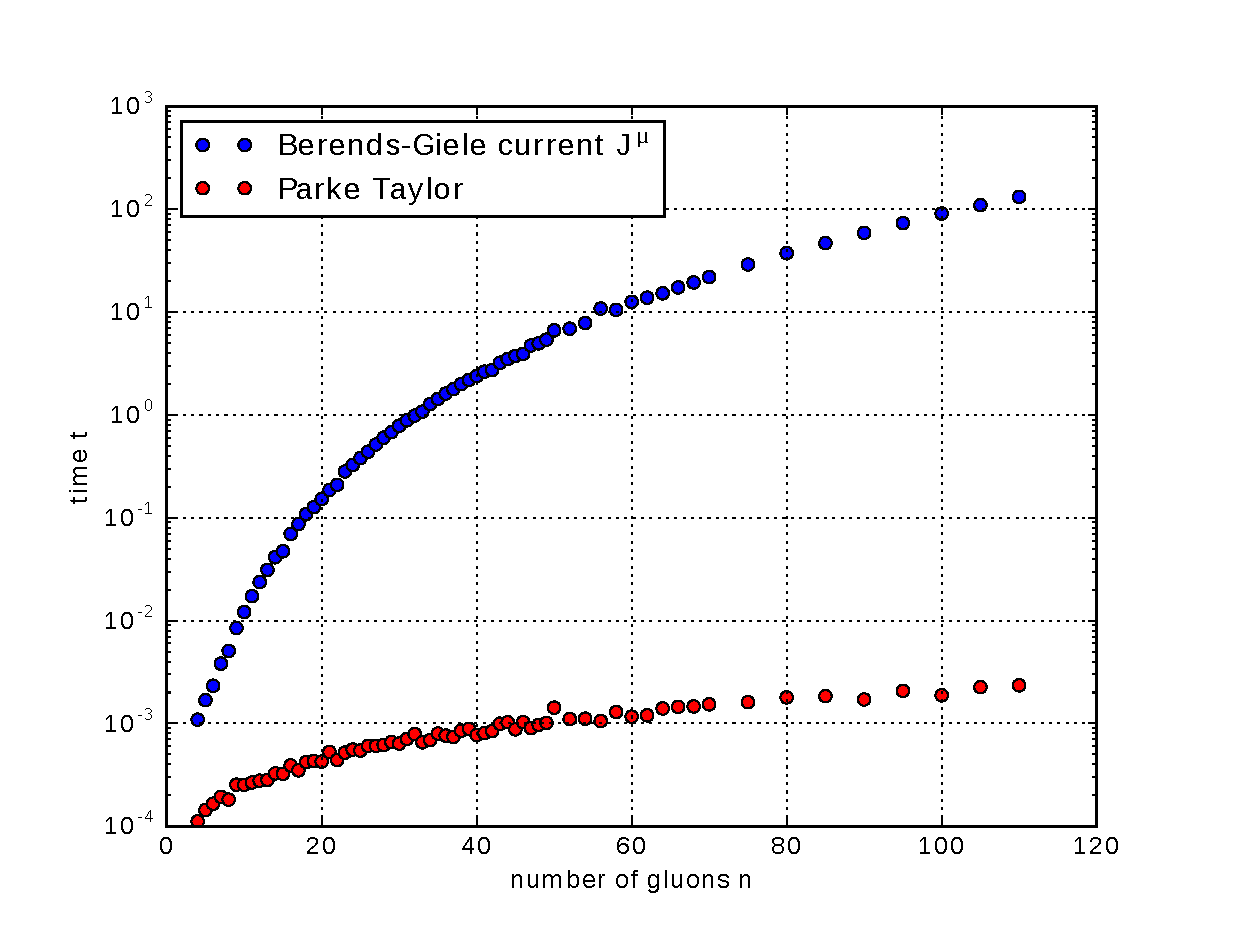
\includegraphics[scale=0.7,natwidth=1079,natheight=359]{comparison.eps}
        \caption{Comparison of the two formulas to calculate tree level partial amplitudes with $n$ gluons. The $x$ axis represents the number of scattering gluons involved in the calculation, whereas the $y$ axis shows the time needed for the calculation on my laptop (an Intel(R) Core(TM) i5-6200U CPU at 2.30GHz with 4 cores. As described in section \ref{sec:parallel} only one of the 4 cores was used in the calculation).}
        \label{fig:compare}
    \end{center}
\end{figure}

An observation I've encountered, was that with increasing number of gluons $n$ the results of the two formulae deviate sometimes by a small amount. For example in the $n=105$ case the results where

\begin{align*}
    A_{BG} &= ( 2.5090994313359261 - 4.4065818656235933 i ) *10^{-6}, \\
    A_{PT} &= ( 2.4904251975961678 - 4.3896288844922791 i ) *10^{-6},
\end{align*}

where $A_{BG}$ and $A_{PT}$ are the amplitudes recieved from the Berends-Giele and the Parke-Taylor formula respectively. These deviations come from rounding errors, when adding a small float number to a float number bigger in many magnitudes. The implementation of the float datatype in most programming languages exhibit that problem \cite{goldberg1991}. My implementation does not handle such problems, since the deviations are in the $10^{-7}$ scale for $n=105$.

\subsection{Further improvements}
\label{sec:improvements}

There are multiple things that can further improve the performance of the Berends-Giele current.

\subsubsection{Parallel processing}
\label{sec:parallel}

Since the main loops in listing \ref{lst:loops} are not dependent of each other, a parallel processing could be taken into account. Each step adds an additional amount to the total current. So if only considering one iteration the inner loops can be processed in any order - ideal for a parallel approach. The improvement would approximately be a factor of the number of CPU cores.

\subsubsection{C loops}
To utilize parallel processing the loops need to be rewritten in C first, because Python uses a GIL (global interpreter lock) mechanism, that prevents multiple parallel threads to run concurrently.

\subsubsection{C arrays}
Each iterative step in the loops do access multiple arrays in reading as well as writing mode. Python arrays as well as NumPy arrays are slow (but convenient) to access single elements at a time. Some NumPy functions are nonetheless as fast as C in iterating over arrays (for example the \code{einsum()} method), but not in the case of how the Berends-Giele current is implemented above. Still there are 3 remaining loops in listing \ref{lst:loops}, where optimisation can be achieved when utilizing C arrays.

\section{Summary}

The Berends-Giele current is a powerful recursive method to calculate general tree level scattering amplitudes in perturbative QCD. On the other hand, the spinor helicity formalism produces very compact results for specific problems such as MHV amplitudes in the form of the Parke-Taylor formula. These formulas where achieved by decomposing the full amplitude into color independent parts, considering only the color component of the Feynman rules to treat color separately. We were able to split the full problem into smaller problems with simpler kinematic properties. These could then be handled recursively.
The implementation was mainly governed by improving the performance which is a heavily language-specific task. A professional implementation would at least incorporate the improvements addressed in section \ref{sec:improvements}. The Berends-Giele current can also be generalised to all Feynman rules - not only the two gluon vertices - to calculate more general amplitudes including quarks in a recursive way (for example $n-2$ gluons and $2$ quarks) \cite{badger2013}.

\newpage

\bibliography{references}
\bibliographystyle{apalike}

\newpage

\appendix
\section*{Appendices}
\addcontentsline{toc}{section}{Appendices}
\renewcommand{\thesubsection}{\Alph{subsection}}

\subsection{QCD Feynman rules}
\label{sec:frules}

The Feynman rules for QCD in Feynman gauge are \cite{mangano99}

\begin{align*}
    \begin{gathered}
        \begin{fmffile}{diagram_3gluon_vertex}
        \fmfframe(0,10)(0,10){
        \begin{fmfgraph*}(30,30)
            \fmfstraight
            \fmfset{arrow_len}{2mm}
            \fmfset{curly_len}{2mm}
            \fmfset{thin}{0.8pt}
            \fmfpen{thin}
            \fmfleft{g1}
            \fmfright{g2,g3}
            \fmf{gluon}{g1,v}
            \fmflabel{$k,a,\mu$}{g1}
            \fmf{gluon}{g3,v}
            \fmflabel{$p,b,\nu$}{g3}
            \fmf{gluon}{g2,v}
            \fmflabel{$q,c,\rho$}{g2}
        \end{fmfgraph*}
-        }
        \end{fmffile}
    \end{gathered}
    &= \frac{i g}{\sqrt{2}} f^{abc} \left[ \eta^{\nu \rho} (p-q)^{\mu} + \eta^{\rho \mu} (q-k)^{\nu} + \eta^{\mu \nu} (k-p)^{\rho} \right], \\
    \begin{gathered}
        \begin{fmffile}{diagram_4gluon_vertex}
        \fmfframe(0,10)(0,10){
        \begin{fmfgraph*}(30,30)
            \fmfstraight
            \fmfset{arrow_len}{2mm}
            \fmfset{curly_len}{2mm}
            \fmfset{thin}{0.8pt}
            \fmfpen{thin}
            \fmfleft{i1,i2}
            \fmfright{o1,o2}
            \fmf{gluon}{i1,v}
            \fmflabel{$d,\sigma$}{i1}
            \fmf{gluon}{i2,v}
            \fmflabel{$a,\mu$}{i2}
            \fmf{gluon}{o2,v}
            \fmflabel{$b,\nu$}{o2}
            \fmf{gluon}{o1,v}
            \fmflabel{$c,\rho$}{o1}
        \end{fmfgraph*}
        }
        \end{fmffile}
    \end{gathered}
    &= -i g^2 \left[
        \begin{array}{l}
            \phantom{+} f^{abe} f^{cde} (\eta^{\mu \rho} \eta^{\nu \sigma} -  \eta^{\mu \sigma} \eta^{\nu \rho}) \\
                     +  f^{ace} f^{bde} (\eta^{\mu \nu}  \eta^{\rho \sigma} - \eta^{\mu \sigma} \eta^{\rho \nu}) \\
                     +  f^{ade} f^{bce} (\eta^{\mu \nu}  \eta^{\sigma \rho} - \eta^{\mu \rho} \eta^{\sigma \nu})
        \end{array}\right], \\
    \begin{gathered}
        \begin{fmffile}{diagram_gluon_fermion_vertex_a}
        \fmfframe(0,10)(15,10){
        \begin{fmfgraph*}(30,30)
            \fmfstraight
            \fmfset{arrow_len}{2mm}
            \fmfset{curly_len}{2mm}
            \fmfset{thin}{0.8pt}
            \fmfpen{thin}
            \fmfright{f1,f2}
            \fmfleft{g1}
            \fmf{gluon}{g1,v}
            \fmflabel{$a,\mu$}{g1}
            \fmf{fermion}{v,f1}
            \fmflabel{$f^{\prime},\bar{\jmath}$}{f1}
            \fmf{fermion}{f2,v}
            \fmflabel{$f,i$}{f2}
        \end{fmfgraph*}
        }
        \end{fmffile}
    \end{gathered}
    &= -\frac{i g \gamma^{\mu} \delta^{f^{\prime}}_{f} }{\sqrt{2}} {(T^a)_i}^{\bar{\jmath}},
    \quad\quad\quad
    \begin{gathered}
        \begin{fmffile}{diagram_gluon_prop}
        \fmfframe(15,10)(15,10){
        \begin{fmfgraph*}(20,25)
            \fmfstraight
            \fmfset{arrow_len}{2mm}
            \fmfset{curly_len}{2mm}
            \fmfset{thin}{0.8pt}
            \fmfpen{thin}
            \fmfright{g1}
            \fmfleft{g2}
            \fmf{gluon,label=$p$}{g2,g1}
            \fmflabel{$a,\mu$}{g2}
            \fmflabel{$b,\nu$}{g1}
        \end{fmfgraph*}
        }
        \end{fmffile}
    \end{gathered}
    = -\frac{i \delta^{ab} \eta^{\mu \nu}}{p^2}, \\
    \begin{gathered}
        \begin{fmffile}{diagram_gluon_fermion_vertex_b}
        \fmfframe(0,10)(15,10){
        \begin{fmfgraph*}(30,30)
            \fmfstraight
            \fmfset{arrow_len}{2mm}
            \fmfset{curly_len}{2mm}
            \fmfset{thin}{0.8pt}
            \fmfpen{thin}
            \fmfleft{f1,f2}
            \fmfright{g1}
            \fmf{gluon}{v,g1}
            \fmflabel{$a,\mu$}{g1}
            \fmf{fermion}{v,f1}
            \fmflabel{$f^{\prime},\bar{\jmath}$}{f1}
            \fmf{fermion}{f2,v}
            \fmflabel{$f,i$}{f2}
        \end{fmfgraph*}
        }
        \end{fmffile}
    \end{gathered}
    &= \frac{i g \gamma^{\mu} \delta^{f^{\prime}}_{f} }{\sqrt{2}} {(T^a)_i}^{\bar{\jmath}},
    \quad\quad\quad
    \begin{gathered}
        \begin{fmffile}{diagram_fermion_prop}
        \fmfframe(15,10)(20,10){
        \begin{fmfgraph*}(20,25)
            \fmfstraight
            \fmfset{arrow_len}{2mm}
            \fmfset{curly_len}{2mm}
            \fmfset{thin}{0.8pt}
            \fmfpen{thin}
            \fmfright{f1}
            \fmfleft{f2}
            \fmf{fermion,label=$p$}{f1,f2}
            \fmflabel{$f,i$}{f2}
            \fmflabel{$f^{\prime},j$}{f1}
        \end{fmfgraph*}
        }
        \end{fmffile}
    \end{gathered}
    = \frac{i \delta^{f^{\prime}}_f \delta^i_j }{p^2}.
\end{align*}

\subsection{Color ordered QCD Feynman rules}
\label{sec:cofrules}

The color ordered Feynman rules for QCD in Feynman gauge are \cite{dixon1996}

\begin{align*}
    \begin{gathered}
        \begin{fmffile}{diagram_co_3gluon_vertex}
        \fmfframe(0,10)(0,10){
        \begin{fmfgraph*}(30,30)
            \fmfstraight
            \fmfset{arrow_len}{2mm}
            \fmfset{curly_len}{2mm}
            \fmfset{thin}{0.8pt}
            \fmfpen{thin}
            \fmfleft{g1}
            \fmfright{g2,g3}
            \fmf{gluon}{g1,v}
            \fmflabel{$k,\mu$}{g1}
            \fmf{gluon}{g3,v}
            \fmflabel{$p,\nu$}{g3}
            \fmf{gluon}{g2,v}
            \fmflabel{$q,\rho$}{g2}
        \end{fmfgraph*}
        }
        \end{fmffile}
    \end{gathered}
    &= \frac{i}{\sqrt{2}} \left[ \eta^{\nu \rho} (p-q)^{\mu} + \eta^{\rho \mu} (q-k)^{\nu} + \eta^{\mu \nu} (k-p)^{\rho} \right], \\
    \begin{gathered}
        \begin{fmffile}{diagram_co_4gluon_vertex}
        \fmfframe(0,10)(0,10){
        \begin{fmfgraph*}(30,30)
            \fmfstraight
            \fmfset{arrow_len}{2mm}
            \fmfset{curly_len}{2mm}
            \fmfset{thin}{0.8pt}
            \fmfpen{thin}
            \fmfleft{i1,i2}
            \fmfright{o1,o2}
            \fmf{gluon}{i1,v}
            \fmflabel{$\sigma$}{i1}
            \fmf{gluon}{i2,v}
            \fmflabel{$\mu$}{i2}
            \fmf{gluon}{o2,v}
            \fmflabel{$\nu$}{o2}
            \fmf{gluon}{o1,v}
            \fmflabel{$\rho$}{o1}
        \end{fmfgraph*}
        }
        \end{fmffile}
    \end{gathered}
    &= \frac{i}{2} \left[ 2\eta^{\mu \rho} \eta^{\nu \sigma} - \eta^{\mu \nu} \eta^{\rho \sigma} - \eta^{\mu \sigma} \eta^{\nu \rho}\right], \\
    \begin{gathered}
        \begin{fmffile}{diagram_co_gluon_fermion_vertex_a}
        \fmfframe(0,10)(15,10){
        \begin{fmfgraph*}(30,30)
            \fmfstraight
            \fmfset{arrow_len}{2mm}
            \fmfset{curly_len}{2mm}
            \fmfset{thin}{0.8pt}
            \fmfpen{thin}
            \fmfright{f1,f2}
            \fmfleft{g1}
            \fmf{gluon}{g1,v}
            \fmflabel{$\mu$}{g1}
            \fmf{fermion}{v,f1}
            \fmflabel{$f^{\prime}$}{f1}
            \fmf{fermion}{f2,v}
            \fmflabel{$f$}{f2}
        \end{fmfgraph*}
        }
        \end{fmffile}
    \end{gathered}
    &= -\frac{i \gamma^{\mu} \delta^{f^{\prime}}_{f} }{\sqrt{2}},
    \quad\quad\quad
    \begin{gathered}
        \begin{fmffile}{diagram_co_gluon_prop}
        \fmfframe(15,10)(15,10){
        \begin{fmfgraph*}(20,25)
            \fmfstraight
            \fmfset{arrow_len}{2mm}
            \fmfset{curly_len}{2mm}
            \fmfset{thin}{0.8pt}
            \fmfpen{thin}
            \fmfright{g1}
            \fmfleft{g2}
            \fmf{gluon,label=$p$}{g2,g1}
            \fmflabel{$\mu$}{g2}
            \fmflabel{$\nu$}{g1}
        \end{fmfgraph*}
        }
        \end{fmffile}
    \end{gathered}
    = -\frac{i \eta^{\mu \nu}}{p^2}, \\
    \begin{gathered}
        \begin{fmffile}{diagram_co_gluon_fermion_vertex_b}
        \fmfframe(0,10)(15,10){
        \begin{fmfgraph*}(30,30)
            \fmfstraight
            \fmfset{arrow_len}{2mm}
            \fmfset{curly_len}{2mm}
            \fmfset{thin}{0.8pt}
            \fmfpen{thin}
            \fmfleft{f1,f2}
            \fmfright{g1}
            \fmf{gluon}{v,g1}
            \fmflabel{$\mu$}{g1}
            \fmf{fermion}{v,f1}
            \fmflabel{$f^{\prime}$}{f1}
            \fmf{fermion}{f2,v}
            \fmflabel{$f$}{f2}
        \end{fmfgraph*}
        }
        \end{fmffile}
    \end{gathered}
    &= \frac{i \gamma^{\mu} \delta^{f^{\prime}}_{f} }{\sqrt{2}},
    \quad\quad\quad
    \begin{gathered}
        \begin{fmffile}{diagram_co_fermion_prop}
        \fmfframe(15,10)(20,10){
        \begin{fmfgraph*}(20,25)
            \fmfstraight
            \fmfset{arrow_len}{2mm}
            \fmfset{curly_len}{2mm}
            \fmfset{thin}{0.8pt}
            \fmfpen{thin}
            \fmfright{f1}
            \fmfleft{f2}
            \fmf{fermion,label=$p$}{f1,f2}
            \fmflabel{$f$}{f2}
            \fmflabel{$f^{\prime}$}{f1}
        \end{fmfgraph*}
        }
        \end{fmffile}
    \end{gathered}
    = \frac{i \delta^{f^{\prime}}_f }{p^2}.
\end{align*}

\subsection{Code}
\label{sec:code}

All code used in this report is open source and can be found in the GitHub repository \cite{github}

\end{document}
